%% Copernicus Publications Manuscript Preparation Template for LaTeX Submissions
%% ---------------------------------
%% This template should be used for the following class files: copernicus.cls, copernicus2.cls, copernicus_discussions.cls
%% The class files, the Copernicus LaTeX Manual with detailed explanations regarding the comments
%% and some style files are bundled in the Copernicus Latex Package which can be downloaded from the different journal webpages.
%% For further assistance please contact the Publication Production Office (production@copernicus.org).
%% http://publications.copernicus.org


%% Differing commands regarding the specific class files are highlighted.


%% copernicus.cls
\documentclass[gmd]{copernicus}

% A few handy shortcuts
\newcommand{\uf}{\ensuremath{\widetilde{u}}}
\newcommand{\vf}{\ensuremath{\widetilde{v}}}
\newcommand{\thetaf}{\ensuremath{\widetilde{\theta}}}
\newcommand{\phif}{\ensuremath{\widetilde{\phi}}}

\begin{document}

\linenumbers

\title{MicroHH 1.0: a computational fluid dynamics code for direct and large-eddy simulation of atmospheric boundary layer flows}


\author[1,2]{Chiel C. van Heerwaarden}
\author[1]{Bart J. H. van Stratum}
\author[3]{Thijs Heus}
\author[4]{Jeremy A. Gibbs}
\author[4]{Evgeni Fedorovich}

\affil[1]{Meteorology and Air Quality Group, Wageningen University, Wageningen, The Netherlands}
\affil[2]{Max Planck Institute for Meteorology, Hamburg, Germany}
\affil[3]{Cleveland State University, Cleveland, OH, USA}
\affil[4]{University of Oklahoma, Norman, OK, USA}

%% The [] brackets identify the author to the corresponding affiliation, 1, 2, 3, etc. should be inserted.



\runningtitle{MicroHH 1.0}

\runningauthor{van Heerwaarden et al.}

\correspondence{Chiel van Heerwaarden\\ (chiel.vanheerwaarden@wur.nl)}



\received{}
\pubdiscuss{} %% only important for two-stage journals
\revised{}
\accepted{}
\published{}

%% These dates will be inserted by the Publication Production Office during the typesetting process.


\firstpage{1}

\maketitle  %% Please note that for the copernicus2.cls this command needs to be inserted after \abstract{TEXT}

\begin{abstract}
This paper describes MicroHH 1.0, a new and freely available (\url{www.microhh.org}) Computational Fluid Dynamical code for the simulation of wall-bounded turbulent flows in the atmosphere using Direct Numerical Simulation and Large-Eddy Simulation. The paper covers the description of the governing equations, their numerical implementation and the parametrizations involved in the code. Furthermore, the paper presents the validation of the dynamical core in the form of convergence tests and conservation tests and comparison of simulations of channel flows and slope flows against well-established models. The full numerical model, including the associated parametrizations for Large-Eddy simulations of high Reynolds number flows, has been tested for a set of cases under stable and unstable conditions, under the Boussinesq and anelastic approximation and with dry and moist convection under stationary and time-varying boundary conditions. The paper presents performance tests showing good scaling from 256 to 32,768 processes. The Graphical Processing Unit (GPU)-enabled version of the code reaches speedups of more than an order of magnitude with respect to the conventional code for a variety of cases.
\end{abstract}

\introduction  %% \introduction[modified heading if necessary]
In this paper we present a description of MicroHH 1.0, a new Computational Fluid Dynamical code for the simulation of wall-bounded turbulent flows, with a focus on those in the atmosphere. MicroHH is a model that can be run both for Direct Numerical Simulations as well as for Large-Eddy Simulations with applications ranging from channel flows to cloud-covered atmospheric boundary layers. The model has been designed and written from scratch with the aim of creating a highly parallel code that is able to run on more than 10,000 processes with the support of modern techniques. MicroHH has been written in C++ and CUDA, in contrast to the majority of its peers, which are mostly written in Fortran 90. The underlying reasons reasons we explain in Section \ref{sec:technical}.

This paper is built up as following: in Section \ref{sec:dyncore}, we provide a full description of the governing equations of the dynamical core and their numerical implementation is discussed in Section \ref{sec:dyncorediscrete}. Subsequently, in Section \ref{sec:parametrizations} we present the added parametrizations and their underlying assumptions. Section \ref{sec:technical} discusses the technical details of the code. This is followed by a series of model tests on validity, accuracy and performance in Section \ref{sec:tests}, followed by a series of test cases based on previous scientific research (Section \ref{sec:casestudies}). After a short description on how to download, compile and run MicroHH (Section \ref{sec:howto}), concluding remarks and future plans close the paper (Section \ref{sec:conclusion}). In order to keep the explanations of mathematical expressions concise, we have included an Appendix with the symbols, their description and their units that are used beyond the scope of a single section.

\section{Dynamical core: governing equations}\label{sec:dyncore}
The dynamical core of MicroHH solves the conservation equations of mass, momentum and energy under the anelastic approximation as presented in \citet{Bannon1996}. In this approximation, the state variables density, pressure and temperature are described as small fluctuations (denoted with a prime in this paper) around their respective reference profiles (denoted with subcript zero) that are a function of height only. This form of the approximation directly simplifies to the Boussinesq equations if the base density $\rho_0$ is assumed to be constant with height. To facilitate the subsequent discussion of the conservation equations, we define the scale height for density $H_\rho$ based on the reference profile
\begin{eqnarray}
H_{\rho} & \equiv & \left( \dfrac{1}{\rho_0} \dfrac{d \rho_0}{dz} \right)^{-1}
\end{eqnarray}

\subsection{Conservation of mass}
The conservation of mass is formulated as
\begin{eqnarray}
\dfrac{\partial \rho_0 u_i}{\partial x_i} & = & \rho_0 \dfrac{\partial u_i}{\partial x_i} + \rho_0 w H_{\rho}^{-1} = 0 \label{eq:consmassa}.
\end{eqnarray}

Under the Boussinesq approximation ($H_{\rho} \rightarrow \infty$), the equation under division by $\rho_0$ simplifies to conservation of volume
\begin{eqnarray}
\dfrac{\partial u_i}{\partial x_i} & = & 0\label{eq:consmassb}
\end{eqnarray}

\subsection{Conservation of momentum and the equation of state}
The momentum equation is written it the flux form, in order to assure the best possible mass and momentum conservation. The hydrostatic balance $dp_0 / dz~=~-\rho_0 g$ has been subtracted to arrive at the perturbation form
\begin{eqnarray}
\nonumber \dfrac{\partial u_i}{\partial t} & = & - \dfrac{1}{\rho_0} \dfrac{\partial \rho_0 u_i u_j}{\partial x_j} 
- \dfrac{\partial}{\partial x_i}\left(\dfrac{p'}{\rho_0}\right) \\
& + & \delta_{i3} g \dfrac{\theta_v'}{\theta_{v0}} + \nu \dfrac{\partial^2 u_i}{\partial x_j^2} + F_i,\label{eq:consmoma}
\end{eqnarray}
where $\delta_{i3}$ is the Kronecker delta and vector $F_i$ represents external forces resulting from parametrizations or large-scale forcings.

The corresponding equation of state is
\begin{eqnarray}
\dfrac{\theta_v'}{\theta_{v0}} & = & \dfrac{p'}{\rho_0 g H_{\rho}} - \dfrac{\rho'}{\rho_0}\label{eq:statea},
\end{eqnarray}
Under the Boussinesq approximation the two equations simplify to
\begin{eqnarray}
\nonumber \dfrac{\partial u_i}{\partial t} & = & - \dfrac{\partial u_i u_j}{\partial x_j} - \dfrac{1}{\rho_0}\dfrac{\partial p^\prime}{\partial x_i} \\
& + & \delta_{i3} g \dfrac{\theta_v'}{\theta_{v0}} + \nu \dfrac{\partial^2 u_i}{\partial x_j^2} + F_i \label{eq:consmomb},\\
\dfrac{\theta_v'}{\theta_{v0}} & = & - \dfrac{\rho'}{\rho_0}\label{eq:stateb}.
\end{eqnarray}

\subsection{Pressure equation}
The equation to acquire the pressure is diagnostic, because density fluctuations are neglected in the conservation of mass in the anelastic equations (Eq. \ref{eq:consmassa}). To simplify the notation, we define function $f \left( u_i \right)$ that contains all right hand side terms of Eq. \ref{eq:consmoma}, except the pressure gradient. To arrive at the equation that allows us to solve for the pressure, we multiply the equation with the base density $\rho_0$ and take its divergence. Conservation of mass ensures that the tendency term vanishes, and an elliptic equation for pressure remains
\begin{eqnarray}
\dfrac{\partial}{\partial x_i} 
\left[ \rho_0 \dfrac{\partial}{\partial x_i} \left( \dfrac{p'}{\rho_0} \right) \right] & = &
\dfrac{\partial \rho_0 f \left( u_i \right)}{\partial x_i}.\label{eq:presa}
\end{eqnarray}
Under the Boussinesq approximation the equation simplifies to
\begin{eqnarray}
\dfrac{\partial^2}{\partial x_i^2} \left( \dfrac{p'}{\rho_0} \right) & = &
\dfrac{\partial f \left( u_i \right)}{\partial x_i}.\label{eq:presb}
\end{eqnarray}
In Section \ref{sec:dyncorediscrete} we explain how these equations are solved.

\subsection{Conservation of an arbitrary scalar}
The conservation equation of an arbitrary scalar $\phi$ can be written in flux form:
\begin{eqnarray}
\dfrac{\partial \phi}{\partial t} & = & - \dfrac{1}{\rho_0} \dfrac{\partial \rho_0 u_j \phi}{\partial x_j} +
\kappa_\phi \dfrac{\partial^2 \phi}{\partial x_j^2} + S_\phi, \label{eq:consscal}
\end{eqnarray}
where $S_\phi$ represents sources and sinks of the variable.

\subsection{Conservation of energy}
MicroHH provides multiple options for the governing equation for energy. Two modes work with potential temperature $\theta$ (dry dynamics) or liquid water potential temperature $\theta_l$ (moist dynamics) with the following conservation equation
\begin{eqnarray}
\dfrac{\partial \theta}{\partial t} & = & - \dfrac{1}{\rho_0} \dfrac{\partial \rho_0 u_j \theta}{\partial x_j} + \kappa_\phi \dfrac{\partial^2 \theta}{\partial x_j^2} + \dfrac{\theta_0}{\rho_0 c_p T_0} Q,
\end{eqnarray}

A third, more simplified mode, is available for dry dynamics under the Boussinesq approximation. Here, the equation of state can be eliminated and the conservation of momentum and energy can be written as
\begin{eqnarray}
\dfrac{\partial u_i}{\partial t} + \dfrac{\partial u_i u_j}{\partial x_j} & = & 
- \dfrac{1}{\rho_0}\dfrac{\partial p'}{\partial x_i} + \delta_{i3} b + \nu \dfrac{\partial^2 u_i}{\partial x_j^2}\label{eq:consmombsimp},\\
\dfrac{\partial b}{\partial t} + \dfrac{\partial b u_j}{\partial x_j} & = & 
\kappa_b \dfrac{\partial^2 b}{\partial x_j^2}\label{eq:consenbsimp}
\end{eqnarray}

With a slight modification to the previous set of equations, it is possible to study slope flows in periodic domains. If we no longer assume that gravity is directed along the z-axis, but instead assume that the domain is under a slope $\alpha$ such that gravity is distributed between the x-axis and z-axis, and assume that the reference buoyancy increases with height with slope $N^2$, the equations are
\begin{eqnarray}
\dfrac{\partial u}{\partial t} + \dfrac{\partial u_j u}{\partial x_j} & = & 
- \dfrac{1}{\rho_0}\dfrac{\partial p'}{\partial x} + \sin(\alpha) b + \nu \dfrac{\partial^2 u}{\partial x_j^2}\label{eq:consuslope},\\
\dfrac{\partial w}{\partial t} + \dfrac{\partial u_j w}{\partial x_j} & = & 
- \dfrac{1}{\rho_0}\dfrac{\partial p'}{\partial z} + \cos(\alpha) b + \nu \dfrac{\partial^2 w}{\partial x_j^2}\label{eq:conswslope},\\
\dfrac{\partial b}{\partial t} + \dfrac{\partial b u_j}{\partial x_j} & = & 
\kappa_b \dfrac{\partial^2 b}{\partial x_j^2} - \left (u\,\sin(\alpha) + w\,\cos(\alpha) \right) N^2\label{eq:consbslope}
\end{eqnarray}

\section{Dynamical core: numerical implementation}\label{sec:dyncorediscrete}
\subsection{Time integration}
The prognostic equations are solved using low-storage Runge-Kutta time integration schemes, where each prognostic variable requires only two three-dimensional fields that we denote in this section with $\phi$ as an arbitrary prognostic variable and $\delta \phi$ as its tendency that is carried on during all stages of the time integration. The code provides two options: a three-stage third-order scheme \citep{Williamson1980} and a five-stage fourth-order scheme \citep{Carpenter1994}. Both can be written in the same generic form in semi-discrete formulation
\begin{eqnarray}
\left( \delta \phi \right)_n & = & f \left( \phi_n \right) + a_n \left( \delta \phi \right)_{n-1} \\
\phi_{n+1} & = & \phi_n + b_n \Delta t \left( \delta \phi \right)_{n},
\end{eqnarray}
where $f$ is a function that represent the computation of all right hand side terms, $a$ and $b$ are the coefficients for the Runge-Kutta method at stage $n$, and $\Delta t$ is the time step. Expression $f \left( \phi_n \right)$ represents thus the actual tendency calculated using for instance Eqs. \ref{eq:consmoma} or \ref{eq:consscal}, whereas $\delta \phi$ is a composite of the actual tendency and those of the previous stages. In low storage form, the tendencies of the previous stage $\left( \delta \phi \right)_{n-1}$ are retained and multiplied with $a_n$ at the beginning of a stage, except for the first stage, where $a_1 = 0$. 

For the third-order scheme the vectors $a$ and $b$ are
\begin{eqnarray}
a & = & \left\{0, -\frac{5}{9}, -\frac{153}{128} \right\}\\
b & = & \left\{\frac{1}{3}, \frac{15}{16}, \frac{8}{15} \right\}
\end{eqnarray}

For the fourth-order scheme the vectors $a$ and $b$ are
\begin{eqnarray}
\nonumber a & = & \left\{0, -\frac{567301805773}{1357537059087},
-\frac{2404267990393}{2016746695238},\right.\\
& & \left. -\frac{3550918686646}{2091501179385},
-\frac{1275806237668}{842570457699} \right\}\\
\nonumber b & = & \left\{\frac{1432997174477}{9575080441755}, \frac{5161836677717}{13612068292357},
\frac{1720146321549}{2090206949498},\right.\\
& & \left. \frac{3134564353537}{4481467310338},
\frac{2277821191437}{14882151754819} \right\}
\end{eqnarray}

Even though the fourth-order scheme has five stages and is thus considerably more expensive than the third order scheme, the truncation error is so much smaller that under many conditions it pays off to use it. We demonstrate this in Section \ref{sec:validationtime}, where we study the conservation properties of the model and the accuracy of the time integration scheme.

\subsection{Grid}
MicroHH is discretized on a staggered Arakawa C-grid, where the scalars are located in the center of a grid cell and the three velocity components at the faces.

MicroHH can work with stretched grids in the vertical dimension. The grid is initialized from vertical profiles that give the location of the cell centres. The locations of the faces are determined consistent with the spatial order of the interpolations that are described in the next section.

\subsection{Building blocks of the spatial discretization}
The spatial operators are based on finite differences. The code supports second-order and fourth-order accurate discretizations following \citet{Morinishi1998, Vasilyev2000}. From Taylor series spatial operators can be derived that form the building blocks of more advanced operators, such as the advection and diffusion operators. In the following subsections we describe the operators and the derived operators. We use only two dimensions for brevity.

We define two second-order interpolation operators, the former with a small stencil and the latter with a wide stencil
\begin{eqnarray}
\phi_{i,j} \approx \widehat{\phi}^{2x }_{i,j} & \equiv & \dfrac{\phi_{i-\frac{1}{2},j} + \phi_{i+\frac{1}{2},j}}{2},\\
\phi_{i,j} \approx \widehat{\phi}^{2xL}_{i,j} & \equiv & \dfrac{\phi_{i-\frac{3}{2},j} + \phi_{i+\frac{3}{2},j}}{2},
\end{eqnarray}
Interpolations are marked with a hat. The superscript indicates the spatial order (2), and the direction ($x$) and has an extra qualifier $L$ when it is taken over a greater distance. The subscript indicates the position on the grid ($i,j$).

The gradient operators, denoted with operator $\delta$, are defined in a similar way
\begin{eqnarray}
\left. \dfrac{\partial \phi}{\partial x}\right|_{i,j} \approx \delta^{2x} \left( \phi \right)_{i,j} & \equiv & \dfrac{\phi_{i+\frac{1}{2},j} - \phi_{i-\frac{1}{2},j}}
                                                                                                                 {   x_{i+\frac{1}{2}}   -    x_{i-\frac{1}{2}  }} \\
\left. \dfrac{\partial \phi}{\partial x}\right|_{i,j} \approx \delta^{2xL} \left( \phi \right)_{i,j}& \equiv & \dfrac{\phi_{i+\frac{3}{2},j} - \phi_{i-\frac{3}{2},j}}
                                                                                                                  {   x_{i+\frac{3}{2}}   -    x_{i-\frac{3}{2}  }}
\end{eqnarray}
We use the Einstein summation in the operators. For instance, the divergence of vector $\left.u_i\right|_{i,j}$ can be written as $\delta^{2x_i}\left( u_i \right)$.
% \begin{eqnarray}
% \delta^{2x} \left( \phi \right)_{i,j} = \dfrac{\phi_{i+\frac{1}{2},j} - \phi_{i-\frac{1}{2},j}}
%                                               {\Delta x}
% \end{eqnarray}
% 
% \begin{eqnarray}
% \delta^{2xL} \left( \phi \right)_{i,j} = \dfrac{\phi_{i+\frac{3}{2},j} - \phi_{i-\frac{3}{2},j}}
%                                                {3\Delta x}
% \end{eqnarray}

The fourth-order operators, written down in the same notation, are defined as
\begin{eqnarray}
\phi_{i,j} \approx \widehat{\phi}^{4x}_{i,j} \equiv \dfrac{- \phi_{i-\frac{3}{2},j} + 9 \phi_{i-\frac{1}{2},j} + 9 \phi_{i+\frac{1}{2},j} - \phi_{i+\frac{3}{2},j}}{16},\label{eq:interp4}
\end{eqnarray}
and a biased one that can by applied in the vicinity of the boundaries. Note that we only write down the bottom boundary (marked with superscript qualifier $b$) for brevity
\begin{eqnarray}
\phi_{i,j} \approx \widehat{\phi}^{4xb}_{i,j} \equiv \dfrac{ 5 \phi_{i-\frac{1}{2},j} + 15 \phi_{i+\frac{1}{2},j} - 5 \phi_{i+\frac{3}{2},j} + \phi_{i+\frac{5}{2},j}}{16}.
\end{eqnarray}

The centered and biased fourth-order gradient operators are
\begin{eqnarray}
\nonumber
\left. \dfrac{\partial \phi}{\partial x}\right|_{i,j} & \approx & \delta^{4x} \left( \phi \right)_{i,j}\\
& \equiv & \dfrac{\phi_{i-\frac{3}{2},j} - 27 \phi_{i-\frac{1}{2},j} + 27 \phi_{i+\frac{1}{2},j} - \phi_{i+\frac{3}{2},j}}
             {       x_{i-\frac{3}{2}}   - 27    x_{i-\frac{1}{2}}   + 27    x_{i+\frac{1}{2}}   -    x_{i+\frac{3}{2}}},
\end{eqnarray}
and

\begin{eqnarray}
\nonumber
\left. \dfrac{\partial \phi}{\partial x}\right|_{i,j} & \approx & \delta^{4xb} \left( \phi \right)_{i,j}\\
& \equiv & \dfrac{-23 \phi_{i-\frac{1}{2},j} + 21 \phi_{i+\frac{1}{2},j} + 3 \phi_{i+\frac{3}{2},j} - \phi_{i+\frac{5}{2},j}}
                 {-23    x_{i-\frac{1}{2}}   + 21    x_{i+\frac{1}{2}}   + 3    x_{i+\frac{3}{2}}   -    x_{i+\frac{5}{2}}}
\end{eqnarray}

% \begin{eqnarray}
% \delta^{4x} \left( \phi \right)_{i,j}  = \dfrac{\phi_{i-\frac{3}{2},j} - 27 \phi_{i-\frac{1}{2},j} + 27 \phi_{i+\frac{1}{2},j} - \phi_{i+\frac{3}{2},j}}
%                                                {24 \Delta x}
% \end{eqnarray}

% \begin{eqnarray}
% \nonumber 
% &&\left. \dfrac{\partial^2 \phi}{\partial x^2}\right|_{i,j} \approx \delta^{4x} \left( \delta^{4x} \left( \phi \right) \right)_{i,j}\\
% \nonumber
% && = \dfrac{1}{576 \left( \Delta x \right)^2} \left( \phi_{i-3,j} - 54 \phi_{i-2,j} + 783 \phi_{i-1,j}\right.\\
% &&  \left. - 1460  \phi_{i,j} + 783 \phi_{i+1,j} - 54 \phi_{i+2,j} + \phi_{i+3,j} \right)
% \end{eqnarray}

\subsection{Advection}
We use the introduced notation to describe the more complex operators and expand them for illustration. The advection term is discretized in the flux form, where $\phi$ is an arbitrary scalar located in the center of the grid cell. In second order, this gives the following discretization
\begin{eqnarray}
\nonumber
\dfrac{\partial u \phi}{\partial x} + \dfrac{\partial v \phi}{\partial y} & \approx & 
\delta^{2x} \left( u \widehat{\phi}^{2x} \right)_{i,j} + \delta^{2y} \left( u \widehat{\phi}^{2y} \right)_{i,j} \\ 
& = & \dfrac{ u_{i+\frac{1}{2},j} \widehat{\phi}^{2x}_{i+\frac{1}{2},j} - u_{i-\frac{1}{2},j} \widehat{\phi}^{2x}_{i-\frac{1}{2},j} }
            { x_{i+\frac{1}{2}} - x_{i-\frac{1}{2}} }\\
& + & \dfrac{ v_{i,j+\frac{1}{2}} \widehat{\phi}^{2y}_{i,j+\frac{1}{2}} - v_{i,j-\frac{1}{2}} \widehat{\phi}^{2y}_{i,j-\frac{1}{2}} }
            { y_{j+\frac{1}{2}} - y_{j-\frac{1}{2}} }
\end{eqnarray}
The discretization of the advection of the velocity components (see Eqs. \ref{eq:consmoma} and \ref{eq:consmomb}) involves extra interpolations as the following example illustrates
\begin{eqnarray}
\dfrac{\partial v u}{\partial x} = \delta^{2x} \left( \widehat{v}^{2y} \widehat{u}^{2x} \right)_{i,j} =
\dfrac{ \widehat{v}^{2y}_{i+\frac{1}{2},j} \widehat{u}^{2x}_{i+\frac{1}{2},j} - \widehat{v}^{2y}_{i-\frac{1}{2},j} \widehat{u}^{2x}_{i-\frac{1}{2},j} }
      { x_{i+\frac{1}{2}} - x_{i-\frac{1}{2}} }\label{eq:advec2u}
\end{eqnarray}

In the standard fourth-order scheme, the scalar advection in flux form is denoted as
\begin{eqnarray}
\nonumber
\left. \dfrac{\partial u \phi}{\partial x} \right|_{i,j} & \approx & \delta^{4x} \left( u \widehat{\phi}^{4x} \right)_{i,j} \\
\nonumber
& = & \left( u_{i-\frac{3}{2},j} \widehat{\phi}^{4x}_{i-\frac{3}{2},j} - 27 u_{i-\frac{1}{2},j} \widehat{\phi}^{4x}_{i-\frac{1}{2},j} \right.\\
\nonumber
&   &\left. + 27 u_{i+\frac{1}{2},j} \widehat{\phi}^{4x}_{i+\frac{1}{2},j} - u_{i+\frac{3}{2},j} \widehat{\phi}^{4x}_{i+\frac{3}{2},j} \right)\\
&   &\slash \left( x_{i-\frac{3}{2}} - 27 x_{i-\frac{1}{2}} + 27 x_{i+\frac{1}{2}} - x_{i+\frac{3}{2}} \right)
\end{eqnarray}
Hereafter, we assume that operator notation is clear and we no longer expand them.

MicroHH has fully energy-conserving fourth order advection schemes \citep{Morinishi1998} available. These consist of interpolation of two energy conserving second-order schemes to eliminate the second-order error
\begin{eqnarray}
% \nonumber
\left. \dfrac{\partial u \phi}{\partial x} \right|_{i,j} & = & \frac{9}{8} \delta^{2x} \left( u \widehat{\phi}^{2x} \right)_{i,j} 
                                                             - \frac{1}{8} \delta^{2xL} \left( u \widehat{\phi}^{2xL} \right)_{i,j}%\\
% \nonumber
% & = & \frac{9}{16} \dfrac{ u_{i+\frac{1}{2},j} \widehat{\phi}^x_{i+\frac{1}{2},j} - u_{i-\frac{1}{2},j} \widehat{\phi}^x_{i-\frac{1}{2},j} }
%                           { x_{i+\frac{1}{2}} - x_{i-\frac{1}{2}} }\\
% & - & \frac{1}{16} \dfrac{ u_{i+\frac{3}{2},j} \widehat{\phi}^{3x}_{i+\frac{3}{2},j} - u_{i-\frac{3}{2},j} \widehat{\phi}^{3x}_{i-\frac{3}{2},j} }
%                           { x_{i+\frac{3}{2}} - x_{i-\frac{3}{2}} }
\end{eqnarray}
Velocity interpolations, such as in Eq. \ref{eq:advec2u}, still need to be performed with fourth-order accuracy (Eq. \ref{eq:interp4}) in order to  be fourth-order accurate (see \citet{Morinishi1998} for details). To illustrate
\begin{eqnarray}
\dfrac{\partial v u}{\partial x} \approx \frac{9}{8} \delta^{2x} \left( \widehat{v}^{4y} \widehat{u}^{2x} \right)_{i,j} 
                                       - \frac{1}{8} \delta^{2xL} \left( \widehat{v}^{4y} \widehat{u}^{2xL} \right)_{i,j}
\end{eqnarray}

\subsection{Diffusion}
We use a mimetic discretisation for the diffusion that can be written as the divergence of a gradient, using the building blocks defined earlier in this section. As this operator is identical in all directions, we write down only one dimension
\begin{eqnarray}
\left. \kappa_\phi \dfrac{\partial^2 \phi}{\partial x^2}\right|_{i,j} & \approx &
\kappa_\phi \delta^{2x} \left( \delta^{2x} \left( \phi \right) \right)_{i,j}\\
% \kappa_\phi \dfrac{\left. \dfrac{\partial \phi}{\partial x}\right|_{i+\frac{1}{2},j} - \left. \dfrac{\partial \phi}{\partial x}\right|_{i-\frac{1}{2},j}}
%                                 {   x_{i+\frac{1}{2},j} -    x_{i-\frac{1}{2},j}}
\left. \kappa_\phi \dfrac{\partial^2 \phi}{\partial x^2}\right|_{i,j} & \approx &
\kappa_\phi \delta^{4x} \left( \delta^{4x} \left( \phi \right) \right)_{i,j}
\end{eqnarray}

On an equidistant grid, this leads to the well-known second-order accurate operator for the second derivate
\begin{eqnarray}
\kappa_\phi \delta^{2x} \left( \delta^{2x} \left( \phi \right) \right)_{i,j} =
\kappa_\phi \dfrac{ \phi_{i-1,j} - 2 \phi_{i,j} + \phi_{i+1,j} }{\left( \Delta x \right)^2},
\end{eqnarray}
whereas for a fourth-order accurate operator, a seven-point stencil is derived
\begin{eqnarray}
\nonumber
&& \kappa_\phi \delta^{4x} \left( \delta^{4x} \left( \phi \right) \right)_{i,j}\\
\nonumber
&& = \dfrac{\kappa_\phi}{576 \left( \Delta x \right)^2} \left( \phi_{i-3,j} - 54 \phi_{i-2,j} + 783 \phi_{i-1,j}\right.\\
&&  \left. - 1460  \phi_{i,j} + 783 \phi_{i+1,j} - 54 \phi_{i+2,j} + \phi_{i+3,j} \right)
\end{eqnarray}
The seven point wide stencil and its properties has been discussed in detail in \citet{Castillo1995}.
% \begin{eqnarray}
% \nonumber
% \left. \kappa_\phi \dfrac{\partial^2 \phi}{\partial x^2}\right|_{i,j} & = & \kappa_\phi
% \left( \left. \dfrac{\partial \phi}{\partial x}\right|_{i-\frac{3}{2},j} 
% - 27 \left. \dfrac{\partial \phi}{\partial x}\right|_{i-\frac{1}{2},j} \right. \\
% \nonumber
% & & \left. + 27 \left. \dfrac{\partial \phi}{\partial x}\right|_{i+\frac{1}{2},j} 
% - \left. \dfrac{\partial \phi}{\partial x}\right|_{i+\frac{3}{2},j} \right)\\
% & & / \left( x_{i-\frac{3}{2}} - 27    x_{i-\frac{1}{2}} + 27    x_{i+\frac{1}{2}} -    x_{i+\frac{3}{2}} \right)
% \end{eqnarray}
\subsection{Pressure}
The pressure solver has to solve Eqs. \ref{eq:presa} and \ref{eq:presb} following the method of \citet{Chorin1968}. This method is a fractional step method that first computes an intermediate velocity component for the next time step based all right hand side terms of the momentum conservation equation Eq. \ref{eq:consmoma}, denoted with a tilde
\begin{eqnarray}
\left. \widetilde{u_i} \right|^{t+1}_{i,j,k} & = & \left. u_i \right|^{t}_{i,j,k} + \Delta t \left. f_i \right|^{t}_{i,j,k}
\end{eqnarray}
The value at the next time step can be computed as soon as the pressure is known with
\begin{eqnarray}
\left. u_i\right|^{t+1}_{i,j,k} & = & \left. \widetilde{u_i} \right|^{t+1}_{i,j,k} - \Delta t \left. \delta^{nx_i}\left( \dfrac{p}{\rho_0}\right)\right|^t_{i,j,k}
\end{eqnarray}
In order to compute the pressure, we multiply the previous equation with the reference density and take its gradient, to arrive at
\begin{eqnarray}
\nonumber \left. \delta^{nx_i} \left( \rho_0 u_i\right) \right|^{t+1}_{i,j,k} & = & 
\left. \delta^{nx_i} \left( \rho_0 \widetilde{u_i} \right) \right|^{t+1}_{i,j,k}\\
& - &  \Delta t \left.\delta^{nx_i} \left[ \rho_0 \delta^{nx_i}\left( \dfrac{p}{\rho_0}\right) \right] \right|^t_{i,j,k}
\end{eqnarray}
The left hand side is the conservation of mass at the next time step, which equals zero (Eq. \ref{eq:consmassa}). Cancellation of the left hand side results in a diagnostic Poisson equation that is the discrete equivalent of Eq. \ref{eq:presa}. Rewriting leads to
\begin{eqnarray}
\dfrac{\left. \delta^{nx_i} \left( \rho_0 \widetilde{u_i} \right) \right|^{t+1}_{i,j,k}}{\Delta t}
& = &  \left. \delta^{nx_i} \left[ \rho_0 \delta^{nx_i}\left( \dfrac{p}{\rho_0}\right) \right] \right|^t_{i,j,k}.
\end{eqnarray}
To simplify the notation, we name the left hand side term $\psi$ and the $p / \rho_0$ term on the right hand side $\pi$. Solving a Poisson equation is a global operation. Because the fields are periodic in the horizontal directions on an equidistant grid and a Poisson equation is linear, we can perform a Fourier transform in the two horizontal directions
\begin{eqnarray}
\widehat{\psi}_{l,m,k} = - k^2_{*n} \widehat{\pi}_{l,m,k} - l^2_{*n} \widehat{\pi}_{l,m,k}
+ \delta^{nz} \left[ \rho_0 \delta^{nz} \left( \widehat{\pi} \right) \right]_{l,m,k},\label{eq:presfourier}
\end{eqnarray}
where Fourier transformed variables are denoted with a hat, the spatial order of the operation with $n$ and the wave numbers in the two horizontal dimensions $x$ and $y$ are $l$ and $m$ respectively; variables $k_*^2$ and $l_*^2$ are the squares of the modified wave numbers
\begin{eqnarray}
-k_{*2}^2 & \equiv & 2 \dfrac{\cos (k \Delta x)}{\left( \Delta x \right)^2} - \dfrac{2}{\left( \Delta x \right)^2}\\
\nonumber
-k_{*4}^2 & \equiv & 2 \dfrac{\cos (3k \Delta x) - 54 \cos (2k \Delta x) + 783 \cos (k \Delta x)}
{576 \left( \Delta x \right)^2}\\
& - & \dfrac{1460}{576 \left( \Delta x \right)^2}
\end{eqnarray}
where the former is the modified wave number for the second-order accurate solver and the latter is the wave number for the fourth-order one. Both expressions fulfill the limit
$\lim_{\Delta x \rightarrow 0} k_{*n}^2 = k^2$, where $n$ is the order of the scheme.

Solving Eq. \ref{eq:presfourier} for $\widehat{\pi}$ requires solving a banded matrix, which is tridiagonal for the second-order solver and hepta-diagonal for the fourth-order solver. For this a standard Thomas-algorithm is used. After the pressure is acquired, inverse Fourier transforms are applied and subsequently the pressure gradient term (see Eqs \ref{eq:consmoma} and \ref{eq:consmomb}) is computed for all three components of the velocity tendency. Note that the solution of this equation does not require a boundary condition for pressure (see \citet{Vreman2014} for details).

\subsection{Boundary conditions}
The lateral boundaries in MicroHH are periodic. The bottom and top boundary conditions can be formulated in their most general form, the Robin boundary condition
\begin{eqnarray}
a \phi_s + b \left.\dfrac{\partial \phi}{\partial z}\right|_s = c,
\end{eqnarray}
which gives the Dirichlet boundary condition when ${a=1,~b=0}$ and the Neumann boundary condition when ${a=0,~b=1}$. 

MicroHH makes use of ghost cells in order to avoid the need of biased schemes for single interpolation or gradient operators near the wall. The values at the ghost cells are derived making use of the boundary conditions following \citet{Morinishi1998}. The ghost cells for the Dirichlet boundary conditions in the second order accurate discretization are
\begin{eqnarray}
\phi_{-\frac{1}{2}} & = & 2 c - \phi_{\frac{1}{2}},
\end{eqnarray}
whereas those for the Neumann boundary condition are
\begin{eqnarray}
\phi_{-\frac{1}{2}} & = & -c \left( - z_{-\frac{1}{2}} + z_{\frac{1}{2}} \right) + \phi_{\frac{1}{2}}
\end{eqnarray}
In case of the fourth-order scheme, we have two ghost cells and therefore a second boundary condition is required. Here we set the third order derivative equal to zero (see \citet{Morinishi1998}). For the Dirichlet boundary condition we then acquire the following expressions for the ghost cells
\begin{eqnarray}
\phi_{-\frac{1}{2}} & = & \dfrac{8 c - 6 \phi_{\frac{1}{2}} + \phi_{\frac{3}{2}}}{3} \\
\phi_{-\frac{3}{2}} & = & 8 c - 6 \phi_{\frac{1}{2}} + \phi_{\frac{3}{2}},
\end{eqnarray}
whereas in case of a Neumann boundary condition we find
\begin{eqnarray}
\phi_{-\frac{1}{2}} & = & -c  \dfrac{z_{i-\frac{3}{2}} - 27 z_{i-\frac{1}{2}} + 27 z_{i+\frac{1}{2}} - z_{i+\frac{3}{2}}}{24} + \phi_{\frac{1}{2}} \\
\phi_{-\frac{3}{2}} & = & -3c \dfrac{z_{i-\frac{3}{2}} - 27 z_{i-\frac{1}{2}} + 27 z_{i+\frac{1}{2}} - z_{i+\frac{3}{2}}}{24} + \phi_{\frac{3}{2}}
\end{eqnarray}

\section{Physical parametrizations}\label{sec:parametrizations}

\subsection{Subfilter-scale model for large-eddy simulation}
With the governing equations described in Section \ref{sec:dyncore} it is possible to resolve the flow until the finest scales. In many applications, such simulations are too costly. In that case, we do large-eddy simulation, where filtered equations are used to describe the largest scales of the flow, whereas the subfilter-scale motions are modeled. Filtering of the anelastic conservation of momentum equation (Eq. \ref{eq:consmoma}), with a tilde to denote filtered variables, leads to 
\begin{eqnarray}
\nonumber \dfrac{\partial \uf_i}{\partial t} & = & - \dfrac{1}{\rho_0} \dfrac{\partial \rho_0 \uf_i \uf_j}{\partial x_j} 
- \dfrac{\partial \pi}{\partial x_i} - \dfrac{1}{\rho_0} \dfrac{\partial \rho_0 \tau_{ij}}{\partial x_j}\\
& + & \delta_{i3} g \dfrac{\thetaf_v'}{\theta_{v0}} + F_i,\label{eq:consmoma_filter}
\end{eqnarray}
In this equation, a new tensor $\tau_{ij}$ is introduced, which is defined as
\begin{eqnarray}
\tau_{ij}  & \equiv & \widetilde{u_i u_j} - \uf_i \uf_j - \frac{1}{3} \left( \widetilde{u_i u_i} - \uf_i \uf_i \right)
\end{eqnarray}
We denote tensor $\tau_{ij}$ as the anisotropic subfilter-scale stress tensor, because the isotropic part of the full stress tensor has been moved to the pressure, to give the modified pressure $\pi$
\begin{eqnarray}
\pi        & \equiv & \dfrac{\widetilde{p}^\prime}{\rho_0} + \frac{1}{3} \left( \widetilde{u_i u_i} - \uf_i \uf_i \right).
\end{eqnarray}
As $\tau_{ij}$ contains the filtered version of a product of unfiltered velocity components, this term needs to be parameterized. MicroHH uses the Smagorinsky-Lilly \citep{Lilly1968} model, in which $\tau_{ij}$ is modeled as
\begin{eqnarray}
\tau_{ij} & = & -\left( K_m + \nu \right) \left( \dfrac{\partial \uf_i}{\partial x_j} + \dfrac{\partial \uf_j}{\partial x_i} \right)
\end{eqnarray}
The eddy-diffusivity $K_m$ 
\begin{eqnarray}
K_m    & = & \lambda^2 \left( 2 S_{ij} S{ij} \right)^\frac{1}{2}
\left(1 - \dfrac{N^2}{Pr_t S^2} \right)^\frac{1}{2}
\end{eqnarray}
is proportional to the magnitude of the strain $S_{ij}$ tensor
\begin{eqnarray}
S_{ij} & \equiv & \frac{1}{2} \left( \dfrac{\partial \uf_i}{\partial x_j} + \dfrac{\partial \uf_j}{\partial x_i} \right)
\end{eqnarray}
 and takes into account the stratification $N^2 \equiv (g/\theta_{v0})/(\partial \thetaf_v / \partial z)$ as the local potential temperature stratification. Length scale  $\lambda$ is the mixing length defined following \citet{Mason1992}
\begin{eqnarray}
\dfrac{1}{\lambda^n} = \dfrac{1}{\left[ \kappa \left(z + z_0 \right) \right]^n} + \dfrac{1}{\left( c_s \Delta \right)^n}
\end{eqnarray}
which is an arbitrary ($n$ can be chosen freely) matching function between the mixing length following wall scaling to that of the subfilter-scale model. Length scale $\Delta \equiv (\Delta x \Delta y \Delta z)^\frac{1}{3}$ relates to the grid spacing. In case of a high-Reynolds number atmospheric large-eddy simulation with an unresolved near-wall flow, the vertical gradients of the horizontal velocity components $\partial \uf_{i,j}/\partial z$  in the strain tensor are replaced with the theoretical gradients predicted from Monin-Obukhov similarity theory. These calculated following Eq. \ref{eq:surf_grad} and explained in detail in Section \ref{sec:surface_model}.

The same approach is followed for all scalars, including the thermodynamic variable
\begin{eqnarray}
\dfrac{\partial \phif}{\partial t} & = & - \dfrac{1}{\rho_0} \dfrac{\partial \rho_0 \uf_j \phif}{\partial x_j} - \dfrac{1}{\rho_0} \dfrac{\partial \rho_0 R_j}{\partial x_j} + \widetilde{S}_\phi, \label{eq:consscal}
\end{eqnarray}
The term $R$ refers to the subfilter flux of $\phif$ and is defined as
\begin{eqnarray}
R_{\phi,j} = \widetilde{u_j \phi} - \uf_j \phif
\end{eqnarray}
Again, the subfilter-scale flux is parameterized as a function of the gradient
\begin{eqnarray}
R_{\phi,j} = - \left( \dfrac{K_m}{Pr_t} + \kappa \right) \dfrac{\partial \phif}{\partial x_j}
\end{eqnarray}
with the turbulent Prandtl number $Pr_t$ set to $\frac{1}{3}$.

\subsection{Surface model}\label{sec:surface_model}
MicroHH provides the option for a surface model that can be used to compute the surface fluxes of the horizontal momentum components and the scalars in flows over rough surfaces at high Reynolds numbers, which is a typical configuration for atmospheric flows. The surface model is entirely built on Monin-Obukhov Similarity Theory (MOST) that relates surface fluxes of variables to their near-surface gradients using empirical functions that take the height $z_1$ divided by the Obukhov length $L$ as a parameter. $L$ is defined as
\begin{eqnarray}
L   & \equiv & - \dfrac{u_*^3}{\kappa B_0};
\end{eqnarray}
it represents the height at which the magnitude of the buoyancy production / destruction of turbulence kinetic energy equals the shear production.

Following MOST, the friction velocity $u_*$ and the momentum fluxes relate to the near surface wind gradient
\begin{eqnarray}
\dfrac{\kappa z_1}{u_*} \dfrac{\partial U}{\partial z}  = 
- \dfrac{\kappa z_1 u_*}{u w} \dfrac{\partial \uf}{\partial z} =
- \dfrac{\kappa z_1 u_*}{v w} \dfrac{\partial \vf}{\partial z} =
\phi_m \left( \dfrac{z_1}{L} \right),\label{eq:surf_grad}
\end{eqnarray}
where $U$ is defined as $\sqrt{\uf^2 + \vf^2}$. These relationships can be integrated from the roughness length $z_{0m}$ to the first model level $z_1$ resulting in 
\begin{eqnarray}
u_* & =  & f_m \left( U_1 - U_0 \right),\\
uw & = & - u_* f_m \left( \uf_1 - \uf_0 \right),\\
vw & = & - u_* f_m \left( \vf_1 - \vf_0 \right),
\end{eqnarray}
with $f_m$ defined as:
\begin{eqnarray}
f_m & \equiv & \dfrac{\kappa}
{ \ln{\left( \dfrac{z_1}{z_{0m}} \right)}
	- \varPsi_m \left( \dfrac{z_1}{L} \right)
	+ \varPsi_m \left( \dfrac{z_{0m}}{L} \right) }
\end{eqnarray}

The exact procedure for scalars is followed, with
\begin{eqnarray}
\dfrac{\kappa z_1 u_*}{\phi w} \dfrac{\partial \phif}{\partial z} =
\phi_h \left( \dfrac{z_1}{L} \right),
\end{eqnarray}
and in integrated form
\begin{eqnarray}
\phi w & = & u_* f_h \left( \phif_1 - \phif_0 \right),
\end{eqnarray}
with
\begin{eqnarray}
f_h & \equiv &
\dfrac{\kappa}
{ \ln{\left( \dfrac{z_1}{z_{0h}} \right)}
	- \varPsi_h \left( \dfrac{z_1}{L} \right)
	+ \varPsi_h \left( \dfrac{z_{0h}}{L} \right) }
\end{eqnarray}

The functions $\phi_m$, $\phi_h$, $\varPsi_m$ and $\varPsi_h$ are empirical and depend on the static stability of the atmosphere. Under unstable conditions we follow \citet{Wilson2001, Wyngaard2010} 
\begin{eqnarray}
\phi_{m,h} & = & \left( 1 + \gamma_{m,h} \left| \dfrac{z_1}{L} \right|^{2/3} \right)^{-1/2}\\
%\phi_h & = & \left( 1 + \gamma_h \left| z/L \right|^{2/3} \right)^{-1/2}\\
\varPsi_{m,h} & = & 3 \ln{\left( \dfrac{1 + \phi_{m,h}^{-1}}{2} \right)} 
%\Psi_m & = & \left( 1 + (3.6 \frac{z}{L})^{2/3} \right)^{-\frac{1}{2}} \\
%\Psi_h & = & \left( 1 + (3.6 \frac{z}{L})^{2/3} \right)^{-\frac{1}{2}} \\
\end{eqnarray}
where $\gamma_m = 3.6$ and $\gamma_h = 7.9$. Under stable conditions we use \citet{Hogstrom1988, Wyngaard2010}
\begin{eqnarray}
\phi_{m,h} & = & 1 + \lambda_{m,h} \dfrac{z_1}{L}\\
\varPsi_{m,h} & = & - \lambda_{m,h} \dfrac{z_1}{L}
\end{eqnarray}
where $\lambda_m = 4.8$ and $\lambda_h = 7.8$.

With the equations above, the surface fluxes, surface values and near-surface gradients can be computed, but only when the Obukhov length $L$ is know. The surface model calculates the Obukhov length by relating the dimensionless parameter $z_1/ L$ to a Richardson number. The exact definition of the Richardson number, and therefore of the solver, depends on the chosen boundary condition in the model. Three possible options are available
\begin{itemize}
	\item Fixed momentum fluxes and a fixed surface buoyancy flux. Both the friction velocity $u_*$ and the surface buoyancy flux $B_0$ are specified. Under these conditions we define the Richardson number $Ri_a$ equal to $z_1/L$; $L$ can be computed directly from expression
	\begin{equation}
	Ri_a \equiv \dfrac{z_1}{L} = - \dfrac{\kappa z B_0}{u_*^3}.
	\end{equation}
	\item A fixed horizontal velocity $u_0$ at the surface and a fixed surface buoyancy flux $B_0$. The friction velocity $u_*$ is unknown. Now,  $L$ needs to be retrieved from the implicit relationship 
	\begin{equation}
	Ri_b \equiv \dfrac{z_1}{L} f_m^3 = - \dfrac{\kappa z B_0}{ \left(U_1 - U_0 \right)^3}.
	\end{equation}
	\item A fixed surface velocity $u_0$ and a fixed surface buoyancy $b_0$. In this boundary condition the surface values for the horizontal velocities and the buoyancy are given and both $u_*$ and the surface buoyancy flux $B_0$ are unknown. $L$ is then retrieved from
	\begin{equation}
	Ri_c \equiv \dfrac{z_1}{L} \dfrac{f_m^2}{f_h} = \dfrac{\kappa z_1 \left(\widetilde{b}_1 - \widetilde{b}_0 \right)}{ \left(U_1 - U_0 \right)^2}
	\end{equation}
\end{itemize}
In case of the two options that need to be solved by iteration, a lookup table is created  with $L$ as a function of Richardson number. The lookup tables have $10^4$ entries, of which 90 percent is spaced uniformly between $z/L = -5$ to $5$. The remaining 10 percent are used to stretch the negative range up to $z/L = -10^4$ to allow for the correct free convection limit.

\subsection{Thermodynamics}

\section{Technical details of the code}\label{sec:technical}
\subsection{Code structure}
MicroHH is written in C++ and uses of elements of object-oriented programming. The model components are written in classes that define the interface. Inheritance is used to allow for specializations of classes. This way of organizing the code has two advantages: it minimizes switches and it allows extension to reside in their own file, which increases code clarity and facilitates the merging of new code. High performance of computational kernels is achieved by executing kernels in their own function, with explicit inclusions of restrict keywords to ensure that fields do not overlap in memory. Furthermore, compiler specific pragmas are used to indicate where code can be vectorized.

\subsection{Parallelization}
The code uses the Message Passing Interface (MPI) in order to run on a large number of processes. The three-dimensional computational domain for a simulation is split into vertically-oriented pencils standing on a two-dimensional grid.

The code distributes the processes over a Cartesian grid using the MPI\_Cart\_create function and uses this grid to detect the IDs of neighboring processes. In order to avoid complex packing routines, we make use of MPI datatypes wherever possible. The MPI calls are written in an interface to prevent that the typical user has to manually write MPI calls.

The Input/Output (IO) is entirely based on MPI-IO, to ensure that three-dimensional fields and two-dimensional cross sections are stored as single files. We have chosen for MPI-IO in order to limit the number of files written by simulations done on a large number of processes and to allow for restarts on a different number of processes. In order to keep complexity of the IO as low as possible, we make use of the MPI\_Sub\_array function in combination with MPI\_File\_write\_all in order to write three dimensional fields and cross sections.

\subsection{External dependencies}
MicroHH depends on three external software tools or libraries. First, it uses the CMake build system for the generation of Makefiles. CMake allows for parallel builds, which minimizes the compilation time. Furthermore, the FFTW3 library \citep{Frigo2005} is used for the computation of Fast-Fourier Transforms. Last, the statistical routines save their output in NetCDF format and therefore rely on UCAR's NetCDF library. In order to run the provided test cases and their output scripts a Python installation including the Numpy and Matplotlib modules is required. Automatic documentation generation can be done using Doxygen, but this is optional.

\section{Validity, accuracy and performance} \label{sec:tests}
\begin{figure}[t]
\vspace*{2mm}
\begin{center}
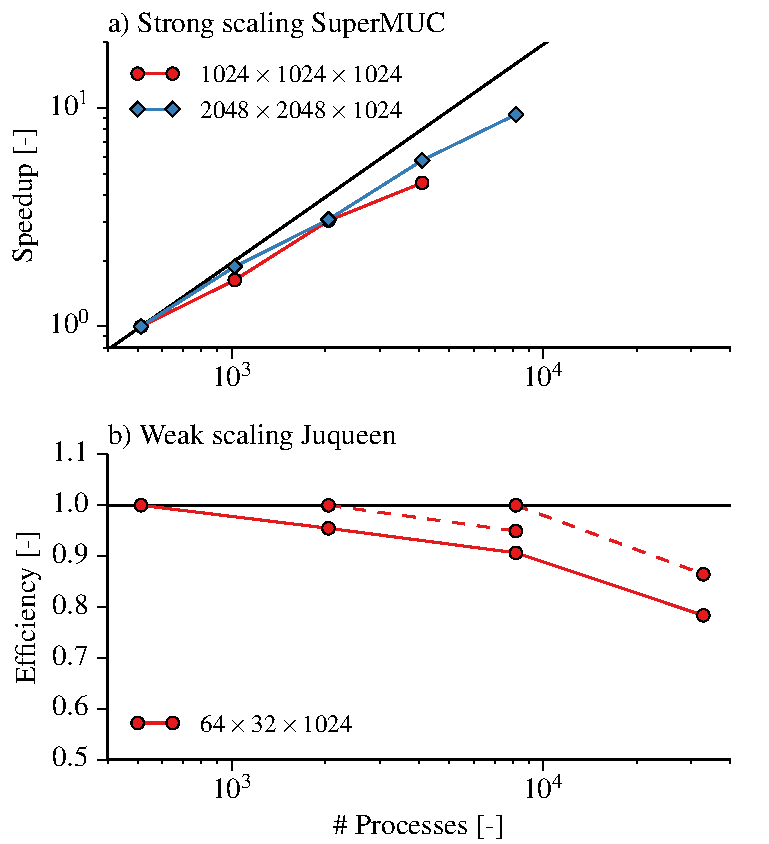
\includegraphics[width=8.3cm]{figs/scaling.pdf}
\end{center}
\caption{Error convergence of the spatial discretization in the two-dimensional Taylor-Green vortex. The dashed black line shows second-order convergence, the dotted black line shows fourth-order convergence.}
\end{figure}
\subsection{Evaluation of the dynamical core}
\subsubsection{Taylor-Green vortex}
Bla.
\begin{figure}[t]
\vspace*{2mm}
\begin{center}
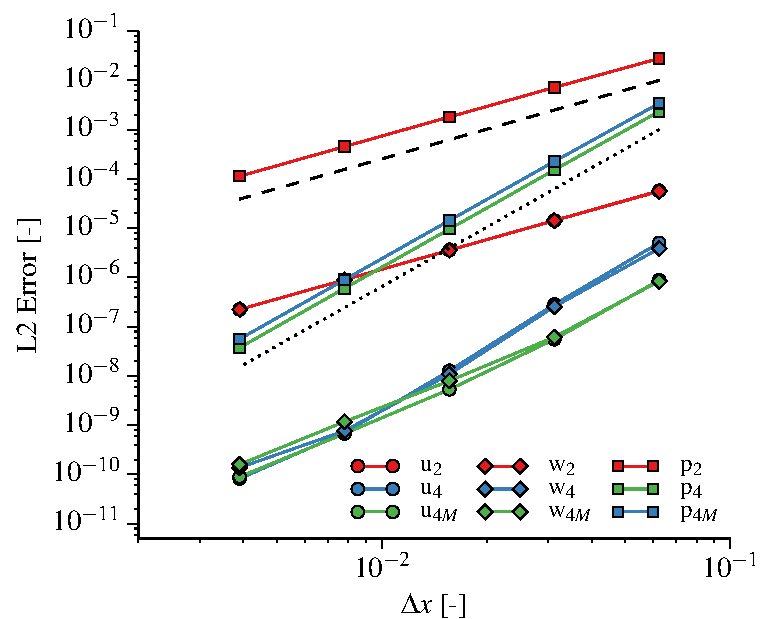
\includegraphics[width=8.3cm]{figs/taylorgreen.pdf}
\end{center}
\caption{Error convergence of the spatial discretization in the two-dimensional Taylor-Green vortex. The dashed black line shows second-order convergence, the dotted black line shows fourth-order convergence.}
\end{figure}

\subsection{Energy conservation and time accuracy}\label{sec:validationtime}
Bla.
\begin{figure}[t]
\vspace*{2mm}
\begin{center}
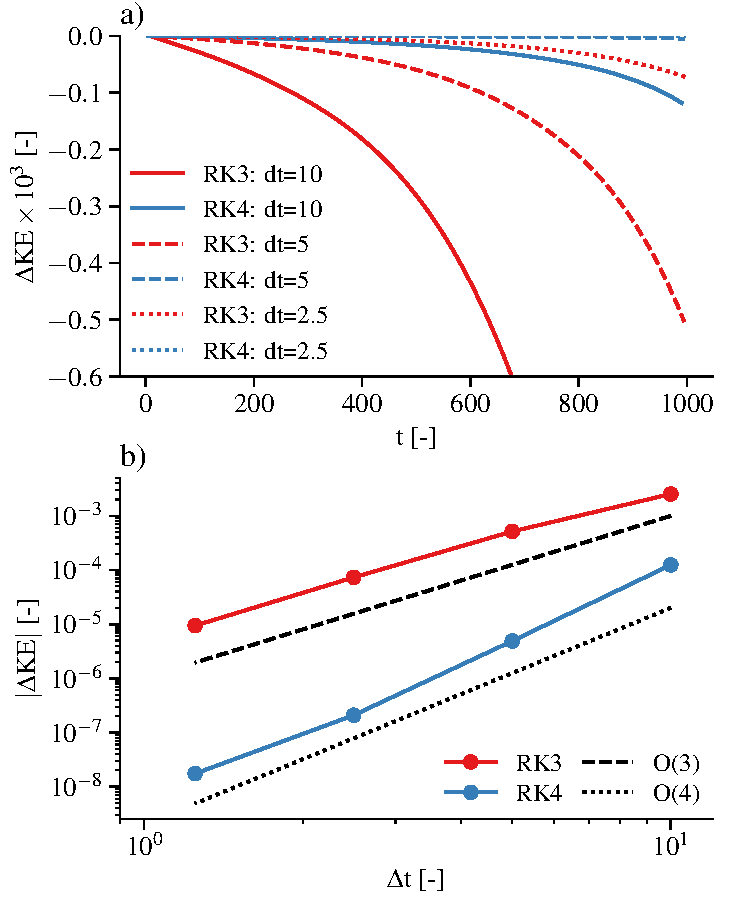
\includegraphics[width=8.3cm]{figs/timeconvergence.pdf}
\end{center}
\caption{Time evolution of the energy loss during 1000 time units of random noise advection for the RK3 and RK4 time integration schemes for three different time steps (a), and error convergence of the temporal discretization for the RK3 and RK4 scheme (b).}
\end{figure}

\subsection{Performance}\label{sec:performance}
\subsubsection{CPU}
\subsubsection{Performance GPU (CUDA) implementation}

Comparison single NVIDIA Quadro K6000 (Cuda 6.5) versus Thunder cluster (2 Intel Xeon E5-2670 CPU's per node, 16 cores per node, Intel 15.01 with OpenMPI 1.8.4). Bomex case (Bxx), with grid dimensions of $64^3$, $128^3$, $256^3$ and $512^2 \times 384$. Moser180 and Moser600 default case from microhh repo. All cases without statistics. 

\begin{table}[t]
\caption{Performance relative to GPU}
\begin{tabular}{rccccc}
\tophline
case & $n$=1 & $n$=16 & $n$=32 & $n$=64   \\
\middlehline
B64  & 18.49 & 1.93 & 1.14 & 0.95 \\
B128 & 28.01 & 2.98 & 1.51 & 0.92 \\
B256 & 27.76 & 3.02 & 1.59 & 0.91 \\
B512 & 29.88 & 3.03 & 1.56 & 0.86 \\
\middlehline
M180 & 21.57 & 2.17 & 1.13 & 0.69 \\
M600 & 22.55 & 2.25 & 1.06 & 0.60 \\
\bottomhline
\end{tabular}
\end{table}


\section{Case studies}\label{sec:casestudies}
\subsubsection{Laminar katabatic flow}


\subsubsection{Channel flow}
The first experiment we compare against data is a neutral channel flow as discussed in MOSER. Strictly speaking, this is an evaluation of the dynamical core of the model, but as the flow is turbulent, we cannot compare it against an analytical solution.

The simulation has a Reynolds-$\tau$ number of 590. SPECS

Figure \ref{fig:moser_velocity}a shows the normalized horizontally-averaged streamwise velocity in panel, and the normalized rms of all three velocity components in Figure \ref{fig:moser_velocity}b. All plotted variables show a perfect match with the data and are indistinguishable from Moser's data. In order to further assess the accuracy of the data, we show the budgets of the variances in Figure \ref{fig:moser_budget}. Also here, the match with the reference data is excellent, which indicates that the whole range of spatial scales in the flow is represented well and that the fourth-order scheme is well able to pick up the details of for instance the disspiation $\epsilon$ that depends on local gradients in the flow.

The findings in the previous paragraph are further corroborated by the spectra shown in Figure \ref{fig:moser_spectra}.  

\begin{figure}[t]
\vspace*{2mm}
\begin{center}
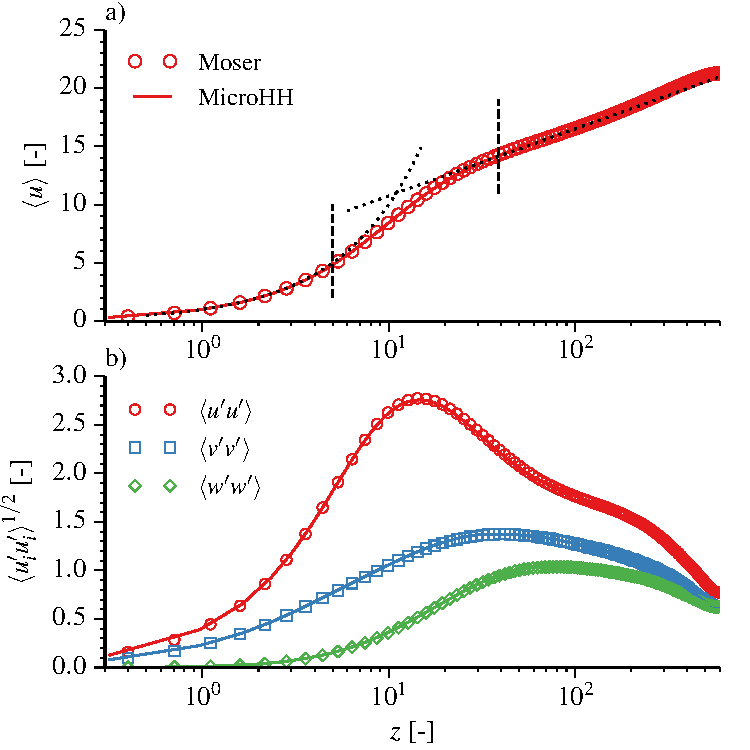
\includegraphics[width=8.3cm]{figs/gmd_m590_umean_var.pdf}
\end{center}
\caption{Moser590. Dashed line = spectra location. $z$ normalized with $u_\tau / \nu$, velocities with $u_\tau^{-1}$.}\label{fig:moser_velocity}
\end{figure}

%% TWO-COLUMN FIGURES
\begin{figure*}[t]
\vspace*{2mm}
\begin{center}
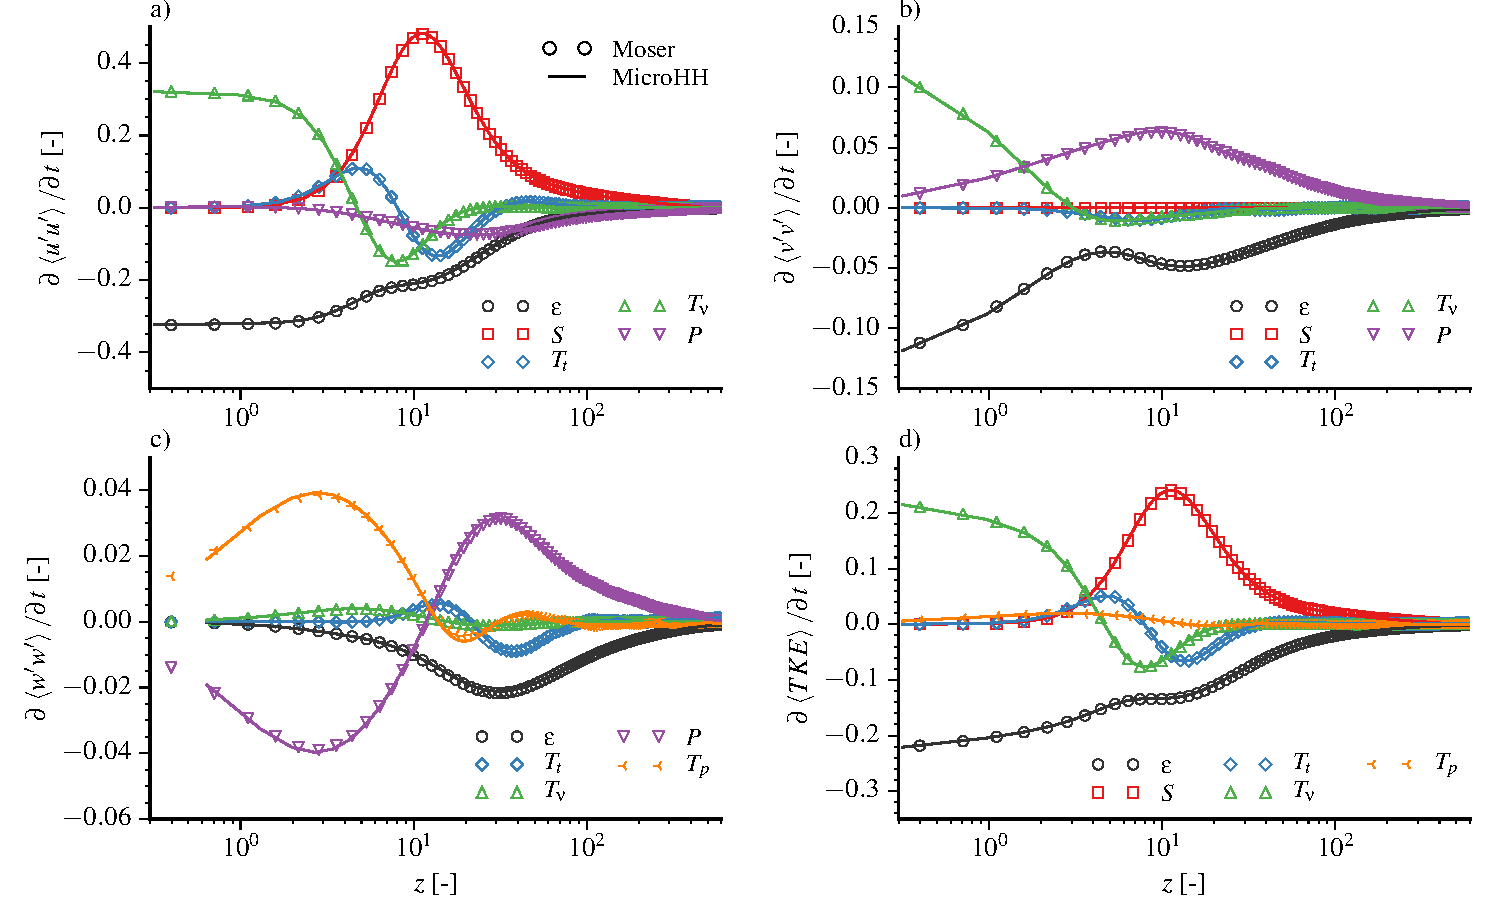
\includegraphics[width=16.6cm]{figs/gmd_m590_turb_budg.pdf}
\end{center}
\caption{Moser590 variance and TKE budgets. $z$ normalized with $u_\tau / \nu$, variances and TKE budget with $\nu / u_\tau^{4}$.}\label{fig:moser_variance}
\end{figure*}

%% TWO-COLUMN FIGURES
\begin{figure*}[t]
\vspace*{2mm}
\begin{center}
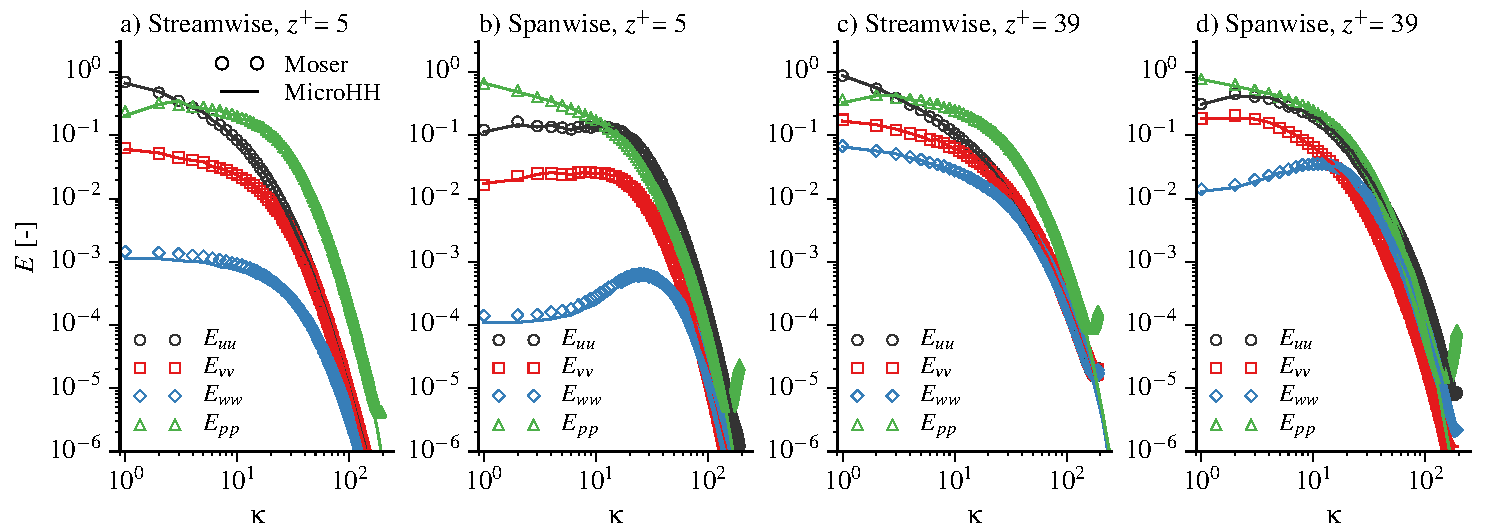
\includegraphics[width=16.6cm]{figs/gmd_m590_spectra_4x1.pdf}\label{fig:moser_spectra}
\end{center}
\caption{Moser590 spectra, velocity spectra are normalized with $u_\tau^{-2}$, pressure spectra with $u_\tau^{-4}$}
\end{figure*}

\subsubsection{Dry CBL}

\subsubsection{BOMEX}

To validate the moist thermodynamics (influence of phase changes on buoyancy) Fig. \ref{fig:bomex} shows the comparison of MicroHH for the BOMEX non-precipitating shallow cumulus LES intercomparison (SIEBESMA), using the resolution from the intercomparison setup (100 m $\times$ 100 m $\times$ 40 m) and a higher resolution (10 m $\times$ 10 m $\times$ 9.375 m) setup. All mean and conditionally sampled statistics are predominantly within one standard deviation of the results from SIEBESMA, except for the cloud and cloud core vertical velocity in the higher resolution setup (STILL LOOKING INTO WHY, T.B.C...). 

\begin{figure*}[t]
\vspace*{2mm}
\begin{center}
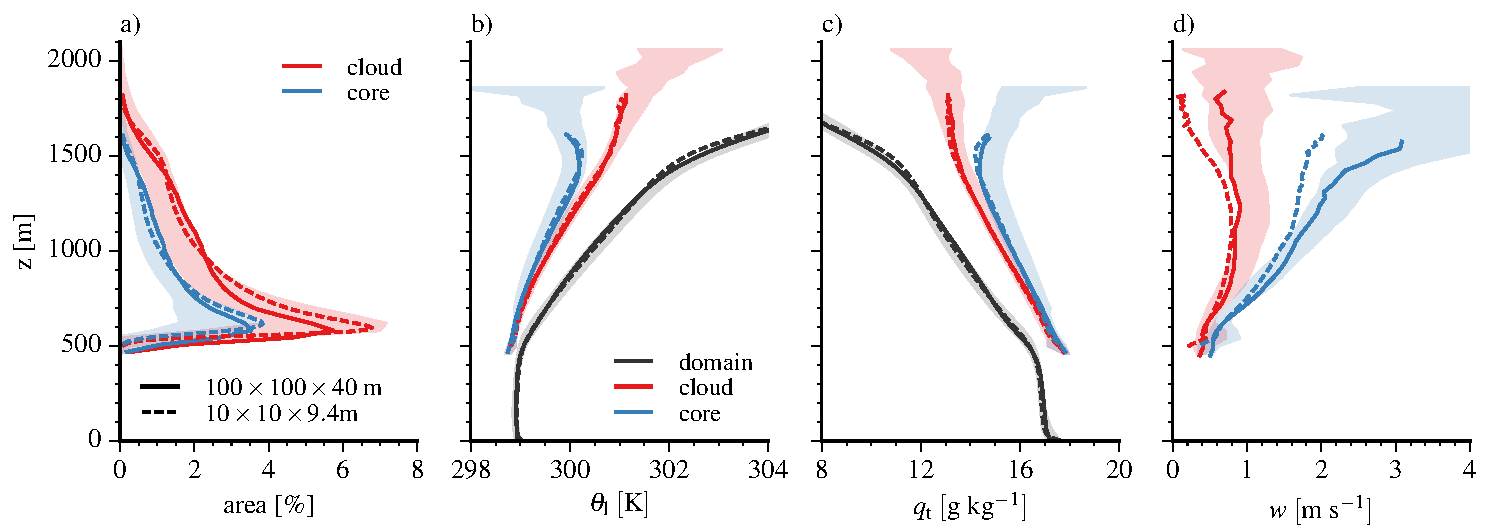
\includegraphics[width=16.6cm]{figs/gmd_bomex_profs.pdf}
\end{center}
\caption{BOMEX LES intercomparison (SIEBESMA). Shown are the domain mean, and conditionally sampled cloud ($q_\mathrm{l} > 0$) and cloud core ($q_\mathrm{l}>0 \ \mathrm{and} \ b-\langle b \rangle > 0$) vertical profiles of (a) area coverage, (b) liquid water potential temperature, (c) total specific humidity and (d) vertical velocity. The results are averaged over t=18000 s -- 21600 s. The shaded area denotes the mean $\pm$ one standard deviation of the participating models from SIEBESMA, the solid and dashed lines the results from MicroHH, using the original (solid) and a higher resolution (dashed) setup.}
\label{fig:bomex}
\end{figure*}

\subsubsection{GABLS1}

The previous examples all focussed on neutral or (conditionally) unstable conditions. As a reference for stable conditions, Fig. \ref{fig:gabls} shows results from the GABLS1 LES intercomparison (BEARE). The result from MicroHH were obtained using the Boussinesq approximation, a centered advection scheme with 4th order accurate interpolations (SECOND ORDER ADVECTION WITH HIGHER ORDER INTERPOLATIONS IS NOT YET DESCRIBED...), and Smagorinsky diffusion using $C_\mathrm{s}$ = 0.XX and a turbulent Prandtl number of XX (JUST TO BE SURE I'LL RE-RUN THESE EXPERIMENTS, RESULTS ARE REALLY OLD...)

\begin{figure*}[t]
\vspace*{2mm}
\begin{center}
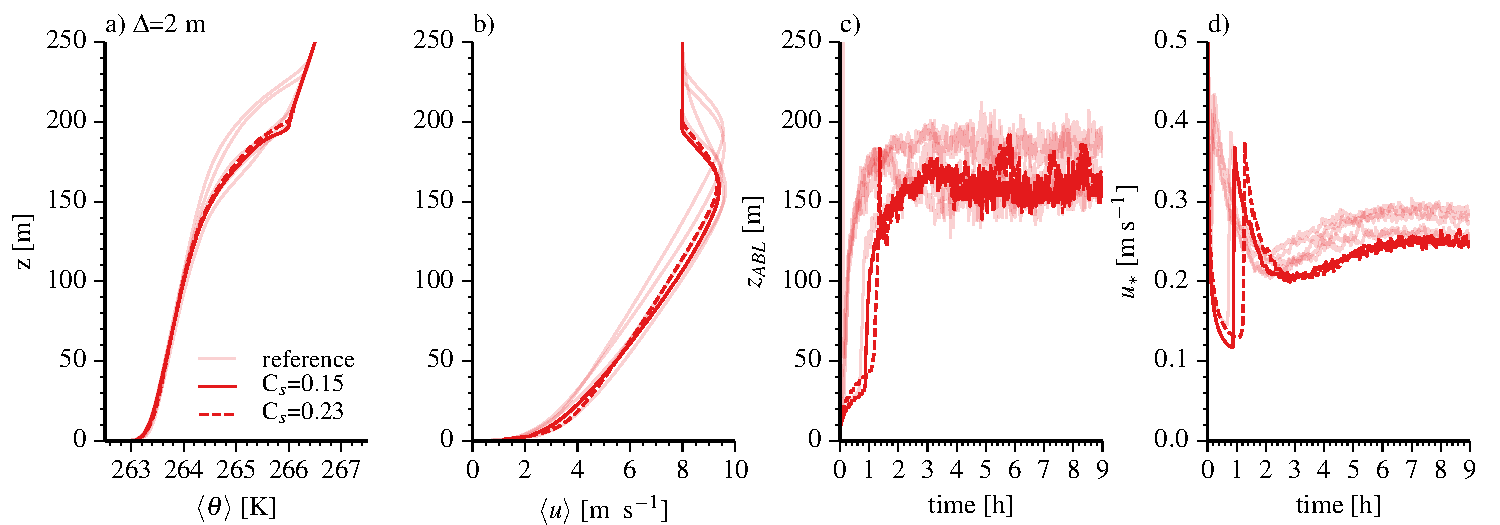
\includegraphics[width=16.6cm]{figs/gmd_gabls_prof_tser.pdf}
\end{center}
\caption{GABLS1 LES intercomparison (BEARE). Shown are the vertical profiles of (a) potential temperature and (b) u-component of the horizontal velocity, and time series of the (c) boundary layer depth and (d) surface friction velocity. The vertical profiles are averages over t=28800 s -- 32400 s. In gray the results from the participating models from BEARE (2 m resolution) are shown, in blue and red the results from MicroHH using a 2 m and 6.25 m grid spacing, respectively. The dotted black line shows the initial conditions.}
\label{fig:gabls}
\end{figure*}

\subsubsection{Katabatic flow}
\subsubsection{Governing equations}

\noindent Katabatic flow (wind) is an atmospheric buoyantly driven boundary-layer flow along a cooled sloping surface in a stratified fluid. We simulate a particular case of katabatic wind that blows along a planar, doubly-infinite slope with the surface cooling prescribed in terms of a spatially and temporally constant surface heat/buoyancy flux. Effects of the Earth rotation on the katabatic wind are neglected, which corresponds to the assumption of a very large Rossby number, and the diffusivities for momentum and temperature are taken equal each other (Prandtl number is assumed to be 1). 

Momentum balance equations for a katabatic flow in the Boussinesq approximation are the following (Fedorovich and Shapiro 2009): 
\begin{eqnarray} \label{GrindEQ__1_} 
\nonumber \frac{\partial u}{\partial t} +u\frac{\partial u}{\partial x} +v\frac{\partial u}{\partial y} +w\frac{\partial u}{\partial z} =-\frac{\partial \pi }{\partial x} +\beta \theta \sin \alpha \\ +\nu \left(\frac{\partial ^{2} u}{\partial x^{2} } +\frac{\partial ^{2} u}{\partial y^{2} } +\frac{\partial ^{2} u}{\partial z^{2} } \right),  
\end{eqnarray} 
\begin{eqnarray} \label{GrindEQ__2_} 
\nonumber \frac{\partial v}{\partial t} +u\frac{\partial v}{\partial x} +v\frac{\partial v}{\partial y} +w\frac{\partial v}{\partial z} =-\frac{\partial \pi }{\partial y} \\+\nu \left(\frac{\partial ^{2} v}{\partial x^{2} } +\frac{\partial ^{2} v}{\partial y^{2} } +\frac{\partial ^{2} v}{\partial z^{2} } \right),  
\end{eqnarray} 
\begin{eqnarray} \label{GrindEQ__3_} 
\nonumber \frac{\partial w}{\partial t} +u\frac{\partial w}{\partial x} +v\frac{\partial w}{\partial y} +w\frac{\partial w}{\partial z} =-\frac{\partial \pi }{\partial z} +\beta \theta \cos \alpha \\ +\nu \left(\frac{\partial ^{2} w}{\partial x^{2} } +\frac{\partial ^{2} w}{\partial y^{2} } +\frac{\partial ^{2} w}{\partial z^{2} } \right),  
\end{eqnarray} 
with the heat balance given by
\begin{eqnarray} \label{GrindEQ__4_} 
\nonumber \frac{\partial \theta }{\partial t} +u\frac{\partial \theta }{\partial x} +v\frac{\partial \theta }{\partial y} + w\frac{\partial \theta }{\partial z} =-\gamma (u\sin \alpha +w\cos \alpha ) \\+ \nu \left(\frac{\partial ^{2} \theta }{\partial x^{2} } + \frac{\partial ^{2} \theta }{\partial y^{2} } + \frac{\partial ^{2} \theta }{\partial z^{2} } \right),
\end{eqnarray}

and mass conservation represented by the continuity equation for an incompressible fluid,
\begin{equation} \label{GrindEQ__5_} 
\frac{\partial u}{\partial x} +\frac{\partial v}{\partial y} +\frac{\partial w}{\partial z} =0.  
\end{equation}
 
\noindent  In the above equations, $u,{\rm \; }v,{\rm \; }w$ are velocity components in the right-hand slope-following Cartesian coordinate system (see Fig.~\ref{Figure_coord}) with $x$, $y$, and $z$ being the upslope, cross-slope, and slope-normal coordinates, respectively, $\pi =[p-p_{e} (z')]/\rho _{r} $ is the normalized pressure perturbation [$p_{e} (z')$ is the environmental pressure, $z'$ is the true vertical coordinate, $\rho _{r} $=const is the reference density value], $\theta =\Theta -\Theta _{e} (z')$ is the potential temperature perturbation, $\gamma =d\Theta _{e} /dz'$=const is the gradient of environmental potential temperature, $\beta =g/\Theta _{r} $ is the buoyancy parameter ($\Theta _{r} $=const is the reference potential temperature value, \textit{g} is the gravitational acceleration), $\alpha $ is the slope angle, $\nu $ is the kinematic viscosity equal to the thermal diffusivity.

\begin{figure}
\centerline{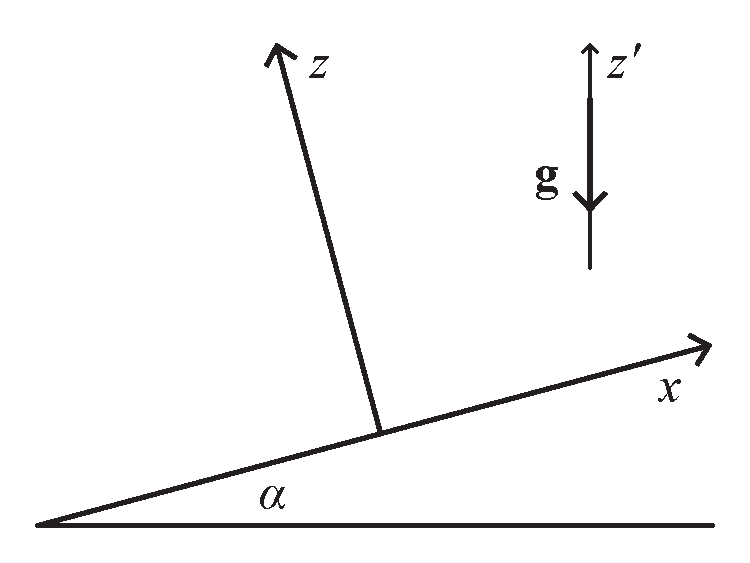
\includegraphics[width=8.3cm]{figs/Figure_coord.pdf}}
\caption{Schematic of the slope-following coordinate system used in simulations of katabatic flows.}
\label{Figure_coord}
\end{figure}

The heat balance equation \eqref{GrindEQ__4_} may be conveniently rewritten in terms of the buoyancy $b\equiv \beta \theta $ as
\begin{eqnarray} \label{GrindEQ__6_} 
\nonumber \frac{\partial b}{\partial t} +u\frac{\partial b}{\partial x} +v\frac{\partial b}{\partial y} +w\frac{\partial b}{\partial z} =-N^{2} (u\sin \alpha +w\cos \alpha )\\+\nu \left(\frac{\partial ^{2} b}{\partial x^{2} } +\frac{\partial ^{2} b}{\partial y^{2} } +\frac{\partial ^{2} b}{\partial z^{2} } \right),  
\end{eqnarray} 

\noindent  where $N=(\beta \gamma )^{1/2} $ is the Brunt-V\"{a}is\"{a}l\"{a} (or buoyancy) frequency.

The lateral boundary conditions for prognostic variables (\textit{u}, \textit{v}, \textit{w}, \textit{b}) and normalized pressure $\pi $ are periodic (the sloping surface is supposed to be doubly infinite along \textit{x} and \textit{y}). The upper boundary conditions (large \textit{z}) are $\partial \varphi /\partial z=0$, where $\varphi $ is any of (\textit{u}, \textit{v}, \textit{w}, \textit{b}), and $\partial \pi /\partial z$ is obtained from \eqref{GrindEQ__3_}. The surface (\textit{z}=0) conditions are no-slip and impermeability (\textit{u}=\textit{v}=\textit{w}=0), with $\partial \pi /\partial z$ obtained from \eqref{GrindEQ__3_}, and $\nu (\partial b/\partial z)=-B_{s} $, where $B_{s} $ is the surface buoyancy flux which also has a meaning of the surface energy production rate.

Results of numerical simulations of the turbulent katabatic flow based on the complete set of governing equations \eqref{GrindEQ__1_} - \eqref{GrindEQ__3_}, \eqref{GrindEQ__5_}, \eqref{GrindEQ__6_} are presented in section 2.

An early milestone in the formal description of katabatic flows was the Prandtl (1942) one-dimensional model for the laminar flow of a viscous stably-stratified fluid along a uniformly cooled sloping surface. In the Prandlt model, the along-slope advection of environmental (mean) temperature balances thermal diffusion, and the along-slope component of buoyancy balances diffusion of along-slope momentum. All other terms in the equations of motion and thermodynamic energy are identically zero, which provides
\begin{equation} \label{GrindEQ__7_} 
b\sin \alpha +\nu \frac{\partial ^{2} u}{\partial z^{2} } =0,  
\end{equation} 
\begin{equation} \label{GrindEQ__8_} 
-N^{2} u\sin \alpha +\nu \frac{\partial ^{2} b}{\partial z^{2} } =0,  
\end{equation} 

\noindent  with the following boundary conditions: $u(0)=0$, $b(0)=b_{s} $ or $\left. -\nu (db/dz)\right|_{z=0} =B_{s} $, and $u\to 0$ and $b\to 0$ as $z\to \infty $. The controlling parameters of the reduced  (Prandtl) problem are $\alpha $, $\nu $, $N$, and either $b_{s} $ or $B_{s} $.  The original solution was obtained by Prandtl for the flow with prescribed surface buoyancy. Here, however, we focus on the Prandtl-model solution for the flow driven by a constant negative surface buoyancy flux. This solution was obtained in Fedorovich and Shapiro (2009) based on the work of Shapiro and Fedorovich (2004). 

Introducing generic length ($L$), velocity ($V$), and buoyancy ($B$) scales, and applying these scales in \eqref{GrindEQ__7_} and \eqref{GrindEQ__8_}, we come to the following non-dimensionalized momentum and buoyancy balance equations of the Prandtl model:
\begin{equation} \label{GrindEQ__9_} 
b_{n} +\frac{\nu V}{L^{2} \sin \alpha B} \frac{\partial ^{2} u_{n} }{\partial z_{n} ^{2} } =0,  
\end{equation} 
\begin{equation} \label{GrindEQ__10_} 
-u_{n} +\frac{\nu B}{L^{2} \sin \alpha N^{2} V} \frac{\partial ^{2} b_{n} }{\partial z_{n} ^{2} } =0,  
\end{equation} 

\noindent with the boundary conditions transforming into $u_{n} (0)=0$, and $u_{n} \to 0$, $b_{n} \to 0$ as $z_{n} \to \infty $, and $\left. (db_{n} /dz_{n} )\right|_{z_{n} =0} =-\frac{B_{s} }{\nu } \frac{L}{B} $.

Defining the length, velocity, and buoyancy scales as
\begin{equation} \label{GrindEQ__11_}
L=\nu ^{1/2} N^{-1/2} \sin ^{-1/2} \alpha ,
\end{equation}
\begin{equation} \label{GrindEQ__12_}
V=\nu ^{-1/2} N^{-3/2} B_{s} \sin ^{-1/2} \alpha ,
\end{equation}
\begin{equation} \label{GrindEQ__13_}
B=\nu ^{-1/2} N^{-1/2} B_{s} \sin ^{-1/2} \alpha ,
\end{equation}
 
\noindent respectively, reduces the dimensionless problem \eqref{GrindEQ__9_}-\eqref{GrindEQ__10_} to
\begin{eqnarray} \label{GrindEQ__14_} 
b_{n} +\frac{\partial ^{2} u_{n} }{\partial z_{n} ^{2} } =0, \\-u_{n} +\frac{\partial ^{2} b_{n} }{\partial z_{n} ^{2} } =0,  
\end{eqnarray} 

\noindent where
\begin{equation} \label{GrindEQ__15_}
z_{n} =z\nu ^{-1/2} N^{1/2} \sin ^{1/2} \alpha ,
\end{equation}
\begin{equation} \label{GrindEQ__16_}
u_{n} =u\nu ^{1/2} N^{3/2} B_{s} ^{-1} \sin ^{1/2} \alpha ,
\end{equation}
\begin{equation} \label{GrindEQ__17_}
b_{n} =b\nu ^{1/2} N^{3/2} B_{s} ^{-1} \sin ^{1/2} \alpha ,
\end{equation}
 
\noindent with the boundary conditions $u_{n} (0)=0$, $\left. (db_{n} /dz_{n} )\right|_{z_{n} =0} =-1$, and $u_{n} \to 0$, $b_{n} \to 0$ as $z_{n} \to \infty $.

Equations \eqref{GrindEQ__14_} have the following analytical solutions (Shapiro and Fedorovich 2004):
\begin{eqnarray} \label{GrindEQ__18_} 
u_{n} =\sqrt{2} \sin (z_{n} /\sqrt{2} )\exp (-z_{n} /\sqrt{2} ),\\b_{n} =\sqrt{2} \cos (z_{n} /\sqrt{2} )\exp (-z_{n} /\sqrt{2} ).  
\end{eqnarray} 


\noindent These solutions were employed for evaluation of the numerical predictions of velocity and buoyancy profiles in a Prandtl-type laminar katabatic flow. Results of the evaluation are presented in section 3.

\section{Turbulent katabatic flow}
\smallskip

\subsection{Simulation settings}
\smallskip
\begin{itemize}
  \setlength{\itemsep}{0pt}
  \setlength{\parskip}{0pt}
  \setlength{\parsep}{0pt}  
  \item Slope angle: $\alpha = 60^{\circ}$
  \item Surface buoyancy flux: $B_{s} $ = $-0.5{\rm\, m}^{\rm 2}\, {\rm s}^{{\rm -3}} $
  \item Brunt-V\"{a}is\"{a}l\"{a} (buoyancy) frequency: $N$ = $1\,{\rm s}^{{\rm -1}}$
  \item Kinematic viscosity/thermal diffusivity:\\$\nu$ = $-0.0001{\rm\, m}^{\rm 2}\, {\rm s}^{{\rm -1}} $
  \item Domain size: ($X{\times}Y{\times}Z$) = 0.64${\rm\, m}\times$0.64${\rm\, m}\times$1.6${\rm\, m}$
  \item Numerical grid dimensions: \\($n_x{\times}n_y{\times}n_z$) = $256 \times 256 \times 640$
  \item Grid structure: uniform (non-stretched) grid in all three directions, with $\Delta x = \Delta y = \Delta z$ = 0.0025${\rm\, m}$
  \item Time step: adaptive
  \item Initial condition: stratified fluid at rest above the slope with zero surface buoyancy flux
  \item Lateral boundary conditions: periodic
  \item Lower boundary conditions: no-slip and impermeability conditions for velocity, surface-flux condition for buoyancy
  \item Upper boundary conditions: free-slip conditions for velocity, zero-gradient condition for buoyancy
\end{itemize}
\subsection{Flow description and simulation results}

Motion starts once the buoyancy flux is applied at the sloping surface. After passing through relatively short transition stage, the flow becomes turbulent. It is characterized  by random, large-amplitude fluctuations of velocity and buoyancy fields in the near-slope core region and shows a quasi-periodic oscillatory behavior at larger distances from the slope. A typical duration of the transition stage in the conducted simulations is about several seconds. Mean profiles of along-slope velocity component  and buoyancy as well as profiles of second-order turbulence statistics, such as kinematic turbulent fluxes of momentum and buoyancy, and velocity-component and buoyancy fluctuation variances, were evaluated by averaging  the simulated flow fields spatially over $X-Y$ planes and temporally over five oscillation periods beyond the transition stage.

For comparison, the same katabatic flow case was reproduced using the numerical code (hereafter referred to FS09) that was employed to simulate turbulent slope flows in Shapiro and Fedorovich (2008) and Fedorovich and Shapiro (2009). In the version of the code used in this comparison study, the time advancement was performed with an Asselin-filtered second-order leapfrog scheme (Durran 1999). The spatial derivatives were approximated by second-order finite-difference expressions on a staggered uniform grid. The Poisson equation for pressure was solved with a fast Fourier transform technique over the $X-Y$ planes and a tri-diagonal matrix inversion method in the slope-normal direction. No-slip and impermeability conditions are applied on the velocity field at the slope surface. Equation \eqref{GrindEQ__3_} was used to formulate a Neumann boundary condition for the pressure at the surface and at the outer boundary of the domain (large $z$). Normal gradients of prognostic variables (velocity components and buoyancy) are set to zero at the outer computational boundary, and periodic boundary conditions are imposed at the $X-Z$ and $Y-Z$ boundaries of the computational domain.

Numerical results obtained with both numerical codes testify that stable environmental stratification in combination with negative surface buoyancy forcing in the katabatic flow leads to an effective suppression of vertical turbulent exchange in the flow region adjacent to the slope. This suppression results in a shallow near-surface sublayer with strong buoyancy gradients (Fig.~\ref{katabatic_b}) capped by a narrow mean-velocity jet with peak velocity located very close to the ground. (Fig.~\ref{katabatic_u}).

\begin{figure}
\centerline{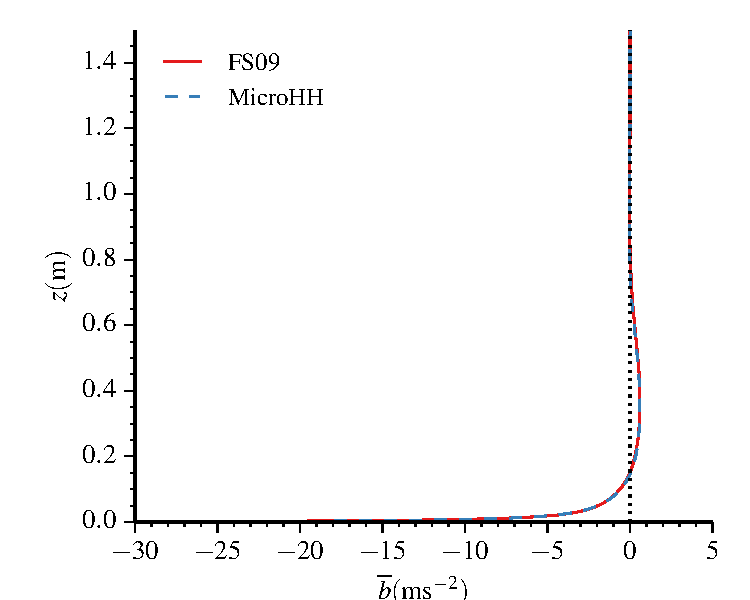
\includegraphics[width=8.3cm]{figs/katabatic_b.pdf}}
\caption{Profile of the mean buoyancy as predicted by MicroHH and FS09.}
\label{katabatic_b}
\end{figure}
 
\begin{figure}
\centerline{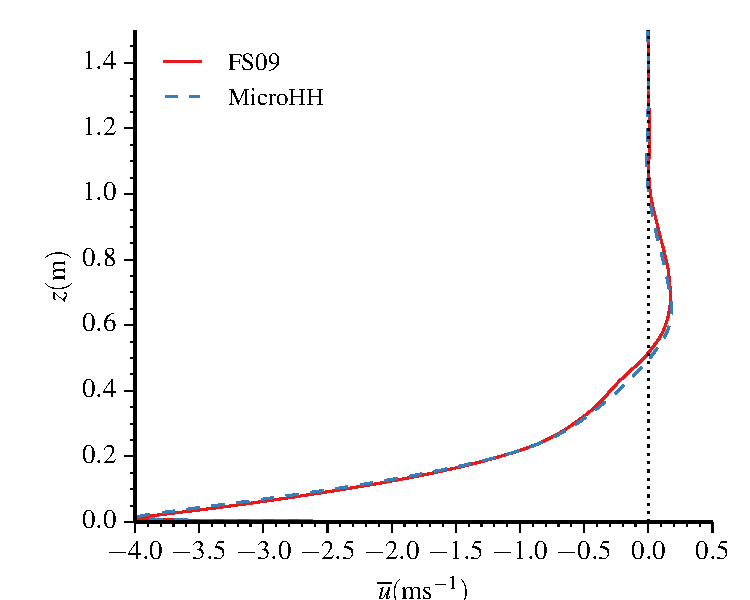
\includegraphics[width=8.3cm]{figs/katabatic_u.pdf}}
\caption{Profile of the mean along-slope velocity as predicted by MicroHH and FS09.}
\label{katabatic_u}
\end{figure}

As revealed by the buoyancy variance profiles in (Fig.~\ref{katabatic_bb}), the buoyancy fluctuations in the simulated katabatic flow attain their maximum magnitude extremely close to the wall, roughly within the region where maximum gradients are observed in the mean buoyancy profiles (Fig.~\ref{katabatic_b}). The drop of $\overline{b'b'}$ beyond the maximum is also rather sharp which means that significant fluctuations of the buoyancy are restricted to a comparatively thin near-wall sublayer.

\begin{figure}
\centerline{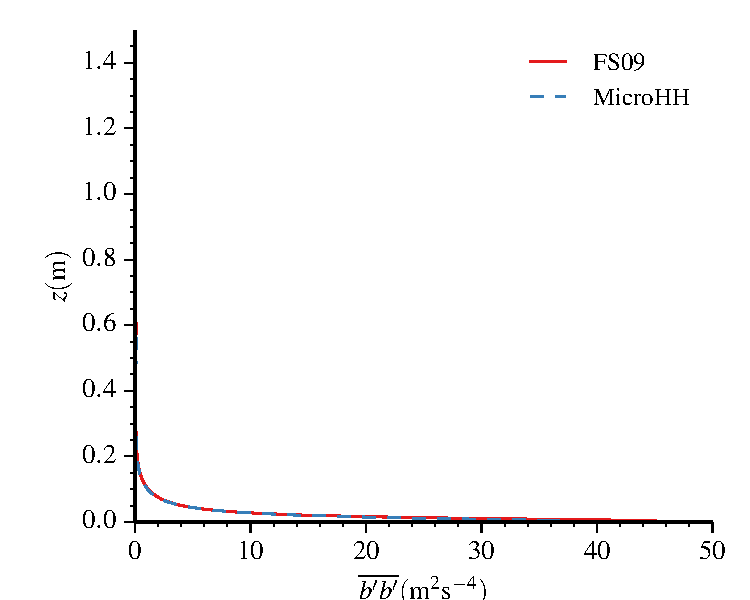
\includegraphics[width=8.3cm]{figs/katabatic_bb.pdf}}
\caption{Profile of the buoyancy variance as predicted by MicroHH and FS09.}
\label{katabatic_bb}
\end{figure}

Along-slope velocity fluctuations of notable magnitudes are distributed over the layer that is about four times thicker than the layer which contains most of the buoyancy variance (compare Fig.~\ref{katabatic_uu} and Fig.~\ref{katabatic_bb}). While the two codes agree with respect to predicting the overall behavior of $\overline{u'u'}$, MicroHH predicts a smoother and stronger maximum of the velocity variance than FS09. The magnitudes of the maxima, though, are fairly close to each other in Fig.~\ref{katabatic_uu}.

\begin{figure}
\centerline{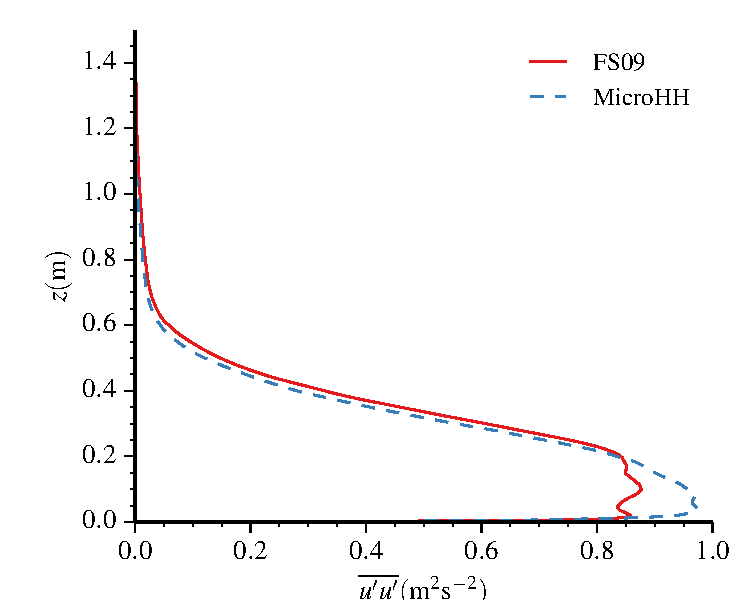
\includegraphics[width=8.3cm]{figs/katabatic_uu.pdf}}
\caption{Profile of the along-slope velocity variance as predicted by MicroHH and FS09.}
\label{katabatic_uu}
\end{figure}

Comparisons of profiles of the cross-slope velocity component variance, $\overline{v'v'}$, and the slope-normal component variance, $\overline{w'w'}$, are presented in Fig.~\ref{katabatic_vv} and Fig.~\ref{katabatic_ww}, respectively.

\begin{figure}
\centerline{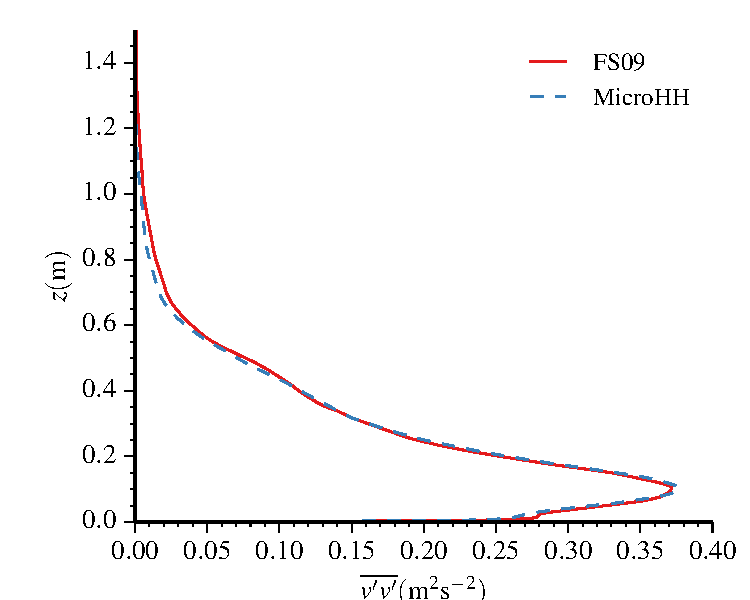
\includegraphics[width=8.3cm]{figs/katabatic_vv.pdf}}
\caption{Profile of the cross-slope velocity variance as predicted by MicroHH and FS09.}
\label{katabatic_vv}
\end{figure}

\begin{figure}
\centerline{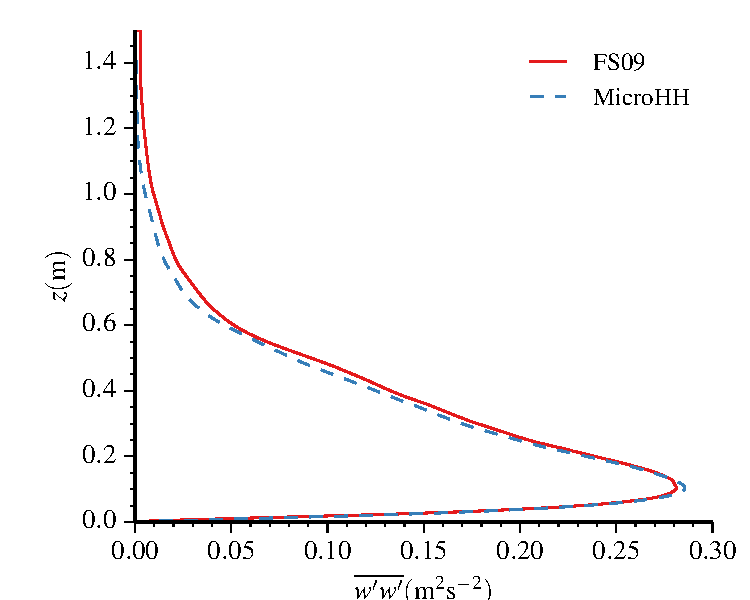
\includegraphics[width=8.3cm]{figs/katabatic_ww.pdf}}
\caption{Profile of the slope-normal velocity variance as predicted by MicroHH and FS09.}
\label{katabatic_ww}
\end{figure}

Profiles of slope-normal fluxes of momentum, $\overline{w'u'}$ (Fig.~\ref{katabatic_wu}), and buoyancy, $\overline{w'b'}$ (Fig.~\ref{katabatic_wb}), indicate that zero crossings in the mean profiles of \textit{b} and \textit{u} are closely co-located with the minima and maxima of the fluxes $\overline{u'w'}$ and $\overline{b'w'}$ except for locations very close to the wall, where molecular effects are important. Typically, molecular fluxes in the simulated flows become negligible at distances from the surface that are significantly smaller than the elevation of the mean velocity maximum (jet elevation).

\begin{figure}
\centerline{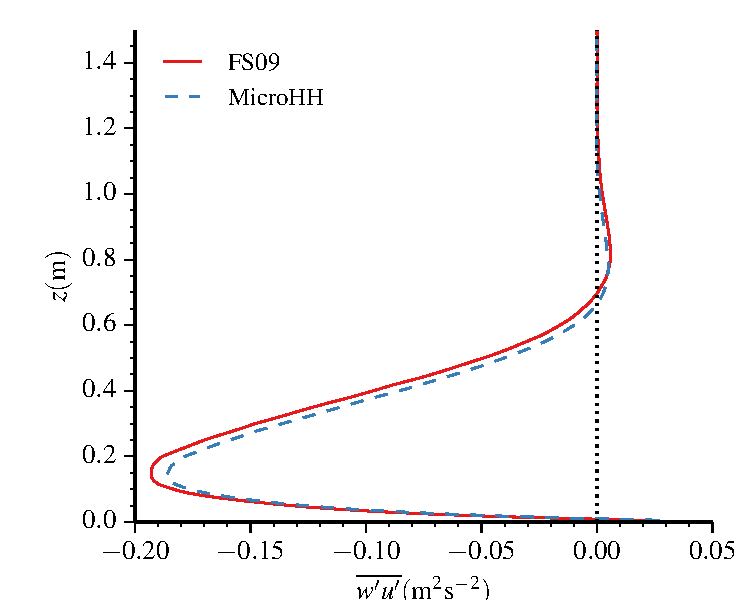
\includegraphics[width=8.3cm]{figs/katabatic_wu.pdf}}
\caption{Profile of the slope-normal turbulent kinematic momentum flux as predicted by MicroHH and FS09.}
\label{katabatic_wu}
\end{figure}
 
\begin{figure}
\centerline{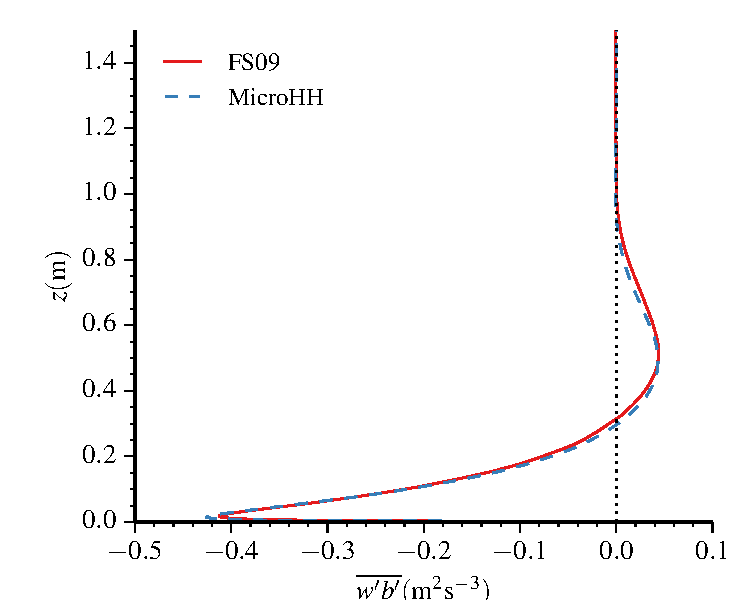
\includegraphics[width=8.3cm]{figs/katabatic_wb.pdf}}
\caption{Profile of the slope-normal turbulent kinematic buoyancy flux as predicted by MicroHH and FS09.}
\label{katabatic_wb}
\end{figure}

Flux profiles shown in Fig.~\ref{katabatic_wu} and Fig.~\ref{katabatic_wb} indicate that there is no region in the flow domain with constancy (even approximate) of either flux with distance from the wall. In more conventional boundary-layer type flows, the existence of height intervals with slowly changing (in the first approximation, constant) momentum and buoyancy fluxes is used as a foundation for similarity analyses and scalings. Such a constant-flux formalism does not apply, at least in a straightforward manner, to the considered katabatic flow case.

\section{Laminar katabatic flow}

\subsection{Simulation settings}

\begin{itemize}
  
  \setlength{\itemsep}{0pt}
  \setlength{\parskip}{0pt}
  \setlength{\parsep}{0pt} 
  \item Slope angle: $\alpha = 30^{\circ}$
  \item Surface buoyancy flux: $B_{s} $ = $-0.005{\rm\, m}^{\rm 2}\, {\rm s}^{{\rm -3}} $
  \item Brunt-V\"{a}is\"{a}l\"{a} (buoyancy) frequency: $N$ = $1\,{\rm s}^{{\rm -1}}$
  \item Kinematic viscosity/thermal diffusivity: \\$\nu$ = $-0.0005{\rm\, m}^{\rm 2}\, {\rm s}^{{\rm -1}} $
  \item Domain size: \\($X{\times}Y{\times}Z$) = 0.015625${\rm\, m}\times$0.001953${\rm\, m}\times$1${\rm\, m}$
  \item Numerical grid dimensions: ($n_x{\times}n_y{\times}n_z$) = $8 \times 1 \times 512$
  \item Grid structure: grid is stretched in the vertical ($z$), with near-surface $\Delta z$ = 0.001${\rm\, m}$, and uniform in $x$ direction  
  \item Time step: adaptive
  \item Initial condition: stratified fluid at rest above the slope with zero surface buoyancy flux
  \item Lateral boundary conditions: periodic
  \item Lower boundary conditions: no-slip and impermeability conditions for velocity, surface-flux condition for buoyancy
  \item Upper boundary conditions: free-slip conditions for velocity, zero-gradient condition for buoyancy
\end{itemize}

\subsection{Flow description and simulation results}

\begin{figure*}[t]
\vspace*{2mm}
\begin{center}
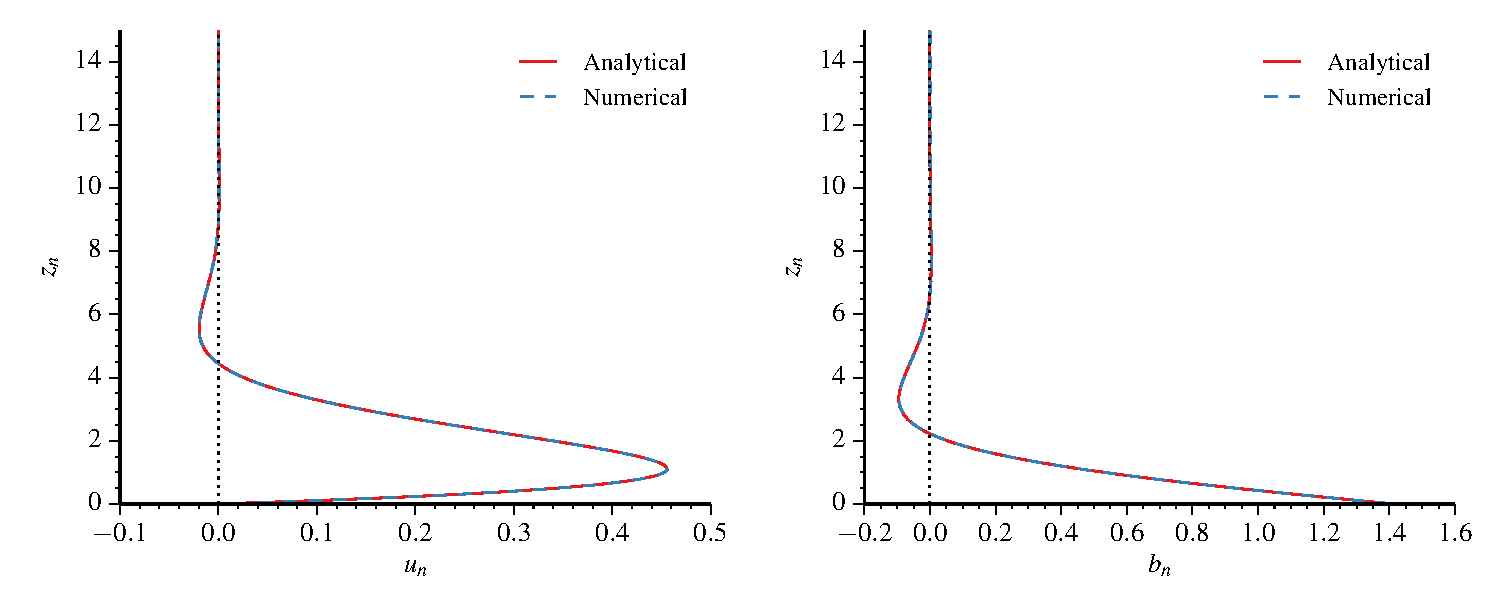
\includegraphics[width=16.6cm]{figs/prandtl.pdf}
\end{center}
\caption{Normalized numerical Prandtl-model solutions for velocity $u$ (left) and buoyancy $b$ (right) compared to their analytical counterparts.}
\label{prandtl}
\end{figure*}

After the negative buoyancy flux is applied at the surface, the fluid, which was initially at rest, goes through the series of decaying oscillations until it reaches the steady state corresponding to the Prandtl model solution. Numerical integration was performed sufficiently long for the oscillation amplitude to become a small fraction of the amplitude of the first oscillation. Computed steady-state profiles of along-slope velocity $u$ and buoyancy $b$ were averaged over $x$ and then normalized using scales \eqref{GrindEQ__11_} - \eqref{GrindEQ__13_}. Comparison of analytical and numerical solutions, which very closely agree with each other, is presented in Fig.~\ref{prandtl}.

\section{How to get MicroHH} \label{sec:howto}

\section{Future plans}
Currently, there are several ongoing projects to extend the model. The physical processes at are currenlty being implemented are microphysics and an interactive land surface model. [BART]

In parallel, preliminary experiments have been performed to include a Domain-Specific Language (DSL) that enables the expression of complex finite difference operators in a simple syntax. The project has shown great potential, for two reasons. First, the DSL reduces the chances of making errors, as the explicit indexing in computational kernels with spatial operators can be omitted. Second, the DSL allows for simple implementation of system specific tuning, such as loop tiling or OpenMP.

\conclusions  \label{sec:conclusion} %% \conclusions[modified heading if necessary]
This paper has explained MicroHH, an new Computational Fluid Dynamics code for simulations of turbulent flows in the atmospheric boundary layer. 

\section{Availability of code and resources}
MicroHH has its own website at \url{http://microhh.org}. Its code is hosted at GitHub and can be accessed either via the website, or directly from 
\url{https://github.com/microhh/microhh}. A selection of visualizations can be viewed at the MicroHH channel at Vimeo \url{https://vimeo.com/channels/817195}.


\section{Appendix}
\begin{table*}[t]
\caption{Overview of used symbols}\label{tab:symbols}
\begin{tabular}{lll}
\tophline
Symbol & Description & Units \\
\middlehline
$\rho_0$ & Reference density & kg~m$^{-3}$\\
$H_\rho$ & Scale height for density & m\\
$u_i$  & Velocity vector $\left( u, v, w \right)$ & m~s$^{-1}$\\
$x_i$  & Position vector $\left( x, y, z \right)$ & m\\
$p^\prime$ & Perturbation pressure & Pa\\
$p_0$ & Reference pressure & Pa\\
$\rho^\prime$ & Perturbation density & kg~m$^{-3}$ \\
$p^\prime$ & Perturbation pressure & Pa\\
$p_0$ & Reference pressure & Pa\\
$\theta_v^\prime$ & Perturbation virtual potential temperature & K\\
$\theta_{v0}$ & Reference virtual potential temperature & K\\
$g$ & Gravity acceleration & m~s$^{-2}$\\
$\nu$ & Kinematic viscosity & m$^{2}$~s$^{-1}$\\
$\kappa$ & Scalar diffusivity & m$^{2}$~s$^{-1}$\\
$F_i$ & External acceleration vector &  m~s$^{-2}$\\
$S$ & External sources and sinks & variable dependent\\
$\theta$ & Potential temperature & K \\
$\theta_l$ & Liquid water potential temperature & K\\
$b$ & Buoyancy & m~s$^{-2}$\\
$T_0$ & Reference absolute temperature & K\\
$Q$ & Heat input & J~m$^{-3}$~s$^{-1}$\\
$\alpha$ & Slope of surface & rad \\
$N$ & Brunt-Vaissala frequency & s\\
\bottomhline
\end{tabular}
\end{table*}


\bibliographystyle{copernicus}
\bibliography{../../misc/refs}
%\bibliography{microhharticle}
\nopagebreak

\smallskip

\noindent Durran, D. R., 1999: \textit{Numerical Methods for Wave Equations in Geophysical Fluid Dynamics}, Springer-Verlag, New York, 465 pp.

\smallskip

\noindent Fedorovich, E., and A. Shapiro, 2009: Structure of numerically simulated katabatic and anabatic flows along steep slopes. \textit{Acta Geophysica},  \textbf{57}, 981-1010.

\smallskip

\noindent Prandtl, L., 1942: \textit{F\"{u}hrer durch die Str\"{o}mungslehre}, Vieweg und Sohn, Braunschweig, 382 pp.

\smallskip

\noindent Shapiro, A., and E. Fedorovich, 2004: Unsteady convectively driven flow along a vertical plate immersed in a stably stratified fluid. \textit{J. Fluid Mech}. \textbf{498}, 333-352.

\smallskip

\noindent Shapiro, A., and E. Fedorovich, 2008: Coriolis effects in homogeneous and inhomogeneous katabatic flows. \textit{Q. J. R. Meteorol. Soc.}, \textbf{134}, 353-370.
\end{document}
